\documentclass[a4paper]{article}

%% Language and font encodings
\usepackage[english]{babel}
\usepackage[utf8x]{inputenc}
\usepackage[T1]{fontenc}

%% Sets page size and margins
\usepackage[a4paper,top=3cm,bottom=2cm,left=3cm,right=3cm,marginparwidth=1.75cm]{geometry}

%% Useful packages
\usepackage{amsmath}
\usepackage{graphicx}
\usepackage[colorinlistoftodos]{todonotes}
\usepackage[colorlinks=true, allcolors=black]{hyperref}
\usepackage[justification=centering]{caption}
\usepackage{comment}
\usepackage{url}

% Code
\usepackage{listings}

\begin{document}

\newcommand{\customlarge}[1]{\noindent \Large{\textbf{#1}}}
\newcommand{\customitalic}[1]{\large{\textbf{\textit{#1}}}}
\newcommand{\avis}[2]{\customlarge{Avis personnel -} \customitalic{#1} \\ #2\\[0.8cm]}
\newcommand*{\escape}[1]{\texttt{\textbackslash#1}}

\newcommand{\customquote}[1]{\guillemotleft {#1} \guillemorright~}

\renewcommand{\contentsname}{Sommaire}


\makeatother

\begin{titlepage}
\newcommand{\HRule}{\rule{\linewidth}{0.5mm}} % Defines a new command for the horizontal lines, change thickness here

\center % Center everything on the page
 
%----------------------------------------------------------------------------------------
%   HEADING SECTIONS
%----------------------------------------------------------------------------------------

\textsc{\LARGE Université de Bordeaux}\\[0.5cm]
\textsc{\large Département Informatique}\\[0.5cm]
\textsc{\large Année 2019-2020}\\[1.5cm]
\textsc{\Large Groupe 21-2}\\[0.2cm] 
\textsc{\large Master 1}\\[0.3cm] 

%----------------------------------------------------------------------------------------
%   TITLE SECTION
%----------------------------------------------------------------------------------------

\HRule \\[0.4cm]
{  \huge \bfseries Projet de Programmation: \\
   \huge \bfseries Génération procédurale de planètes sphériques\\[0.4cm] 
   \Large \bfseries Analyse des besoins
% Title of your document
\HRule \\[1.5cm]
 
%----------------------------------------------------------------------------------------
%   AUTHOR SECTION
%----------------------------------------------------------------------------------------

\begin{minipage}{0.4\textwidth}
\begin{center} \large
\emph{Client:}\\
David \textsc{Renault}\\
~\\
\emph{Auteurs:}\\
Rémi \textsc{Barbosa}\\
Benjamin \textsc{Darmet}\\
Marc \textsc{Cerutti}\\
Sofian \textsc{Antri}\\
Tsiory \textsc{Rakotoarisoa}\\
\end{center}
\end{minipage}
~
}

% If you don't want a supervisor, uncomment the two lines below and remove the section above
%\Large \emph{Author:}\\
%John \textsc{Smith}\\[3cm] % Your name

%----------------------------------------------------------------------------------------
%   DATE SECTION
%----------------------------------------------------------------------------------------

% {\large \today}\\[2cm] % Date, change the \today to a set date if you want to be precise

%----------------------------------------------------------------------------------------
%   LOGO SECTION
%----------------------------------------------------------------------------------------


%----------------------------------------------------------------------------------------

\vfill % Fill the rest of the page with whitespace

\end{titlepage}

% ------------------------ END OF TITLEPAGE ------------------------
\newpage

\tableofcontents

\newpage

\section{Présentation du projet}

En informatique, la génération dite procédurale est la création de contenu numérique (modèle 3D, animation, son, musique,...) à une très grande échelle et de manière automatisée. Elle doit répondre à un ensemble de règles qui sont définies par des algorithmes.\\
\par
Nous cherchons à mettre en place au sein de ce projet, un outil permettant de générer procéduralement et de visualiser des planètes (une à la fois) dans un but ludique (se balader pour le plaisir d'admirer et explorer, découvrir un nouvel environnement). Chaque planète est représentée par une sphère géodésique (divisée en faces) statique dont les faces colorées témoignent de la présence de différents terrains, tels que des océans, des reliefs, des déserts, des plaines etc. Un exemple est visible sur la figure \ref{exemple}. La planète aura un rendu "low-poly", désignant un style graphique avec peu de polygones et donc volontairement peu de détails pour des raisons d'optimisation mais aussi d'esthétique. Une fois la planète générée, il sera possible de la visualiser par une vue à 360° en orbite autour de la planète. Cette vue s'accompagnera d'un outil de zoom afin d'obtenir par la suite une fois très proche, un changement d'orientation du plan pour pouvoir observer l'horizon en première personne, vue humaine, sans déplacement.

\begin{figure}[!h]
    \begin{center}
        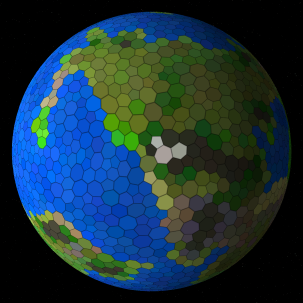
\includegraphics[scale=1]{img/planete.png}
        \caption{Exemple de planète générée procéduralement\protect\footnotemark}
        \label{exemple}
    \end{center}
\end{figure}

\footnotetext{\href{https://experilous.com/1/blog/post/procedural-planet-generation}{https://experilous.com, Procedural Planet Generation Posted on September 30, 2014 by Andy Gainey}}

\newpage
\section{Analyse de l'existant}

\subsection{Algorithmes de génération de sphère}

\subsubsection{Subdivision d'un icosaèdre : icosphére}

Il existe différentes méthodes pour générer une sphère à face polygonale. La toute première est la subdivision à plusieurs reprises d'un  icosaèdre pour obtenir une géode. Un icosaèdre est un polyèdre composé de  12 sommets et 20 triangles équilatéraux (visibile figure  \ref{figure0}). La géode quant à elle est un polyèdre convexe inscrit dans une sphère dont il réalise une approximation. Pour obtenir cette géode, on réalise une subdivision des triangles composant l'icosaèdre en  4 triangles plus petits. On répète cette opération plusieurs fois afin d'obtenir la surface désirée. On peut voir le résultat après 2 subdivisions consécutives sur la figure \ref{figure1}.\\
\\
L'utilisation de cette approche permet d'obtenir une position des points régulière mais aussi une décomposition de la sphère en triangle de même taille sans appliquer d'autres algorithmes supplémentaires (Comme Voronoï ou Delaunay qui sont expliqués plus bas). Il s'agit de la méthode standard. Il est possible d'appliquer cette subdivision sur les uv-spheres et les cubesphéres, mais les polygones ne seront pas identiques, et donc leur taille non plus. Pour plus d'informations, voir la référence \cite{SongHoAhn}. Il est néanmoins possible de partir directement de points et de les relier par la suite. C'est le cas de l'utilisation de la sphère de Fibonacci.\\

\begin{figure}[!h]
    \begin{center}
        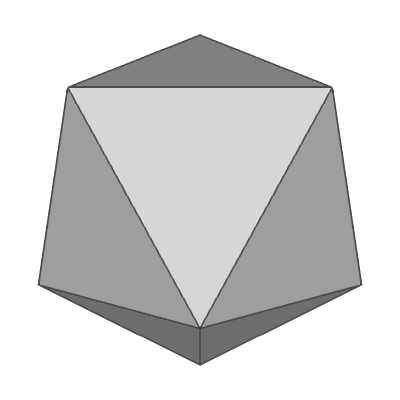
\includegraphics[width=0.2\linewidth]{img/sphere/gl_sphere05.png}
        \caption{Icosaèdre\protect\footnotemark}
        \label{figure0}
    \end{center}
\end{figure}

\footnotetext{\href{http://www.songho.ca/opengl/gl_sphere.html}{http://www.songho.ca/, OpenGL Sphere, 2018 by Song Ho Ahn, Accessed January 2020}}

\begin{figure}[!h]
    \begin{center}
        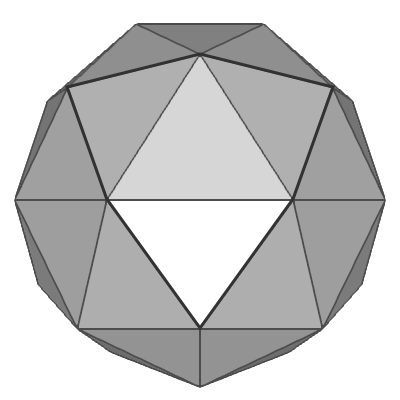
\includegraphics[width=0.2\linewidth]{img/sphere/gl_sphere06-2.png} 
        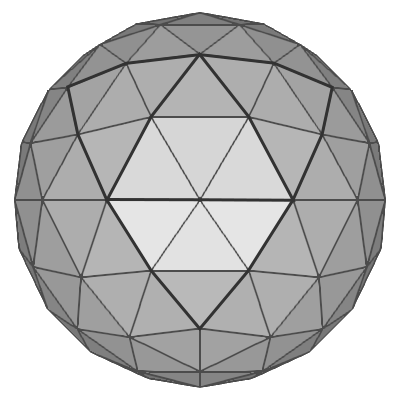
\includegraphics[width=0.2\linewidth]{img/sphere/gl_sphere07-2.png} 
        \caption{Subvidision à 2 reprises d'un icosaèdre.\protect\footnotemark}
        \label{figure1}
    \end{center}
\end{figure}

\footnotetext{\href{http://www.songho.ca/opengl/gl_sphere.html}{http://www.songho.ca/, OpenGL Sphere, 2018 by Song Ho Ahn, Accessed January 2020}}

\subsubsection{Sphère de Fibonacci}

Une sphère de Fibonnacci est la représentation d'une sphère par dispersion de points (voir figure \ref{fibosphere}). Différents algorithmes peuvent être utilisés pour générer cette répartition de points de manière plus ou moins égale. Il y a par exemple celui de la répulsion electrostatique. Il consiste à partir d'une distribution arbitraire des points à appliquer un algorithme de répulsion ponctuelle, dans lequel tous les points se repoussent les uns des autres. On fait alors tourner l'algorithme jusqu'à un certain critère de convergence, autrement dit quand la distribution nous convient. Pour plus d'informations voir \cite{PointDistribution}.
\begin{figure}[!h]
    \begin{center}
        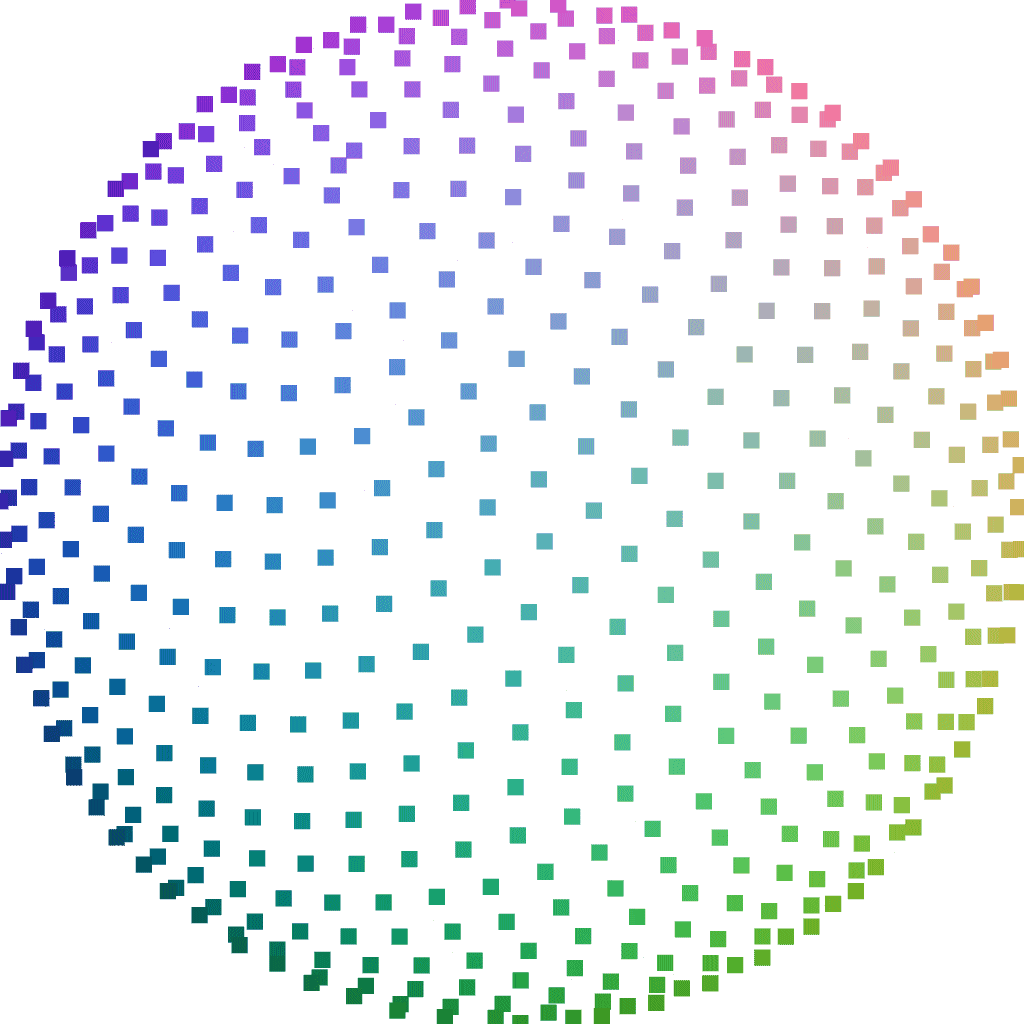
\includegraphics[width=0.5\linewidth]{img/sphere/fibonacci_sphere.png}
    \end{center}
        \caption{Sphère de Fibonacci \protect\footnotemark}
        \label{fibosphere}
\end{figure}

\footnotetext{\href{https://www.redblobgames.com/x/1842-delaunay-voronoi-sphere/}{https://www.redblobgames.com, Delaunay + Voronoi on a sphere
Posted on March 10, 2019 by RedBlobGames, Accessed January 2020}}


Une fois la répartition des points obtenue, il est nécessaire de les relier afin d'obtenir une première version d'une sphère. On peut alors utiliser le tout premier algorithme : La triangulation de Delaunay. Cette triangulation consiste à relier tous les points d'un plan P, tel qu'aucun point de P n'est à l'intérieur du cercle circonscrit d'un des triangles formés. On peut bien sûr étendre cette définition à un espace en 3 dimensions. On parle alors de sphères circonscrites. La sphère finale obtenue est celle de la figure \ref{delaunay}.

\begin{figure}[!h]
    \begin{center}
        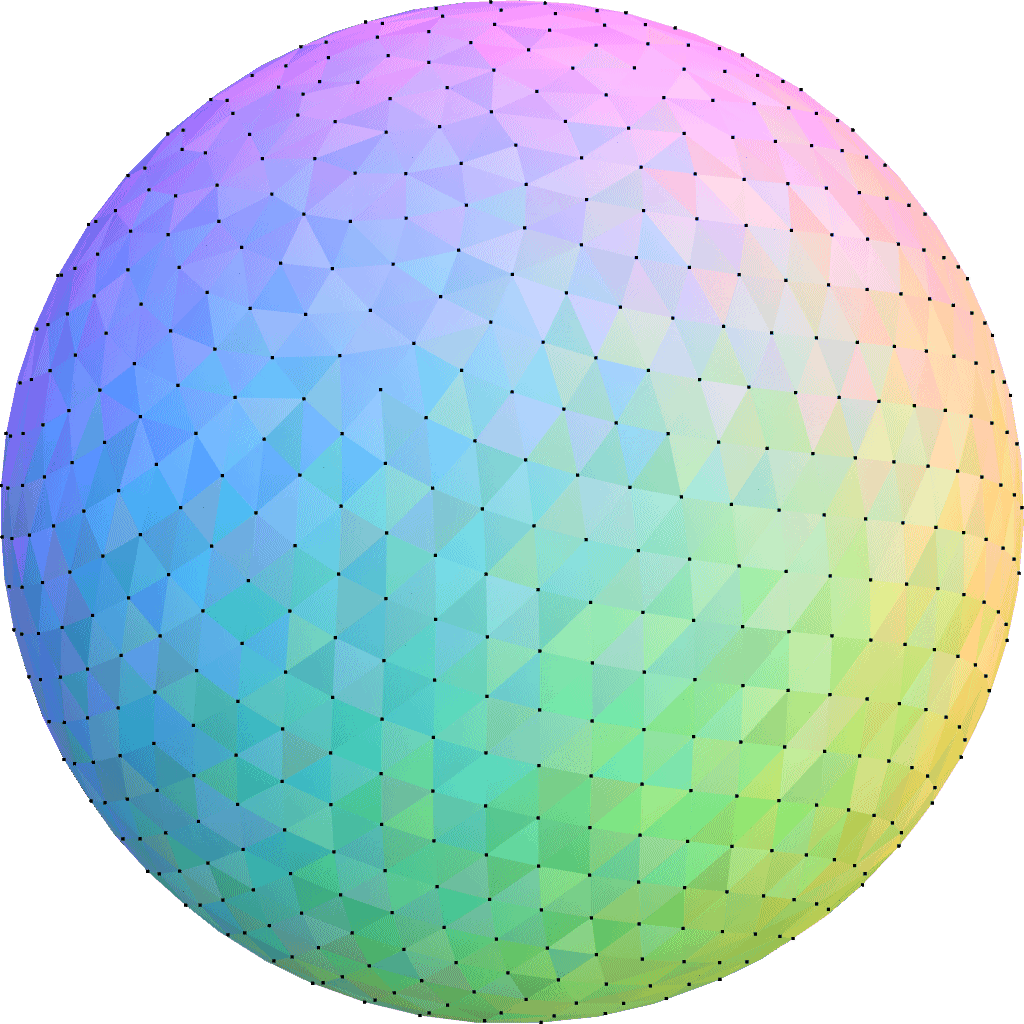
\includegraphics[scale=0.2]{img/sphere/fibonacci-sphere-delaunay.png}
        \caption{Résultat de la triangulation de Delauney pour une sphère\protect\footnotemark}
        \label{delaunay}
    \end{center}
\end{figure}

\footnotetext{\href{https://www.redblobgames.com/x/1842-delaunay-voronoi-sphere/}{https://www.redblobgames.com, Delaunay + Voronoi on a sphere
Posted on March 10, 2019 by RedBlobGames}}

Il est alors facile d'appliquer le diagramme de Voronoï par la suite. Ce diagramme consiste à un pavage (découpage) du plan en cellules. Chaque cellule contient un "germe", représenté par un point, dont la cellule en représente sa zone d'influence. Les sommets du diagramme de Voronoï sont les centres des cercles circonscrits des triangles obtenus par la triangulation de Delaunay. Les arêtes du diagrammes quant à elles sont les médiatrices des arêtes de la triangulation de Delaynay. On peut voir la superposition d'un diagramme de Voronoï et de la triangulation de Delaunay à la figure \ref{superposition}. L'application sur une sphère est présentée à la figure \ref{voronoi}.  Pour plus de détails, il est possible de voir \cite{RedBlobGames}.

\begin{figure}[!h]
    \begin{center}
        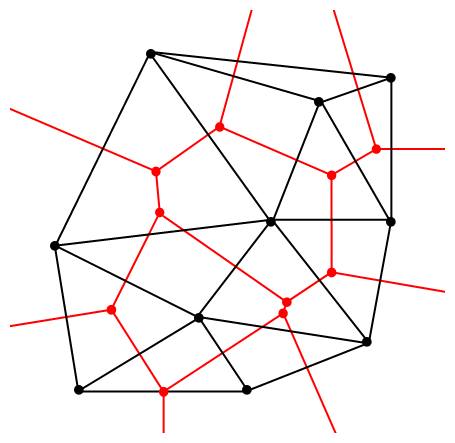
\includegraphics[scale=0.5]{img/Delaunay_Voronoi.png}
        \caption{Superposition d’un diagramme de Voronoï (en rouge) et de la triangulation de Delaunay (en noir).\protect\footnotemark}
        \label{superposition}
    \end{center}
\end{figure}

\footnotetext{\href{https://www.redblobgames.com/x/1842-delaunay-voronoi-sphere/}{https://www.redblobgames.com, Delaunay + Voronoi on a sphere
Posted on March 10, 2019 by RedBlobGames}}

\begin{figure}[!h]
    \begin{center}
        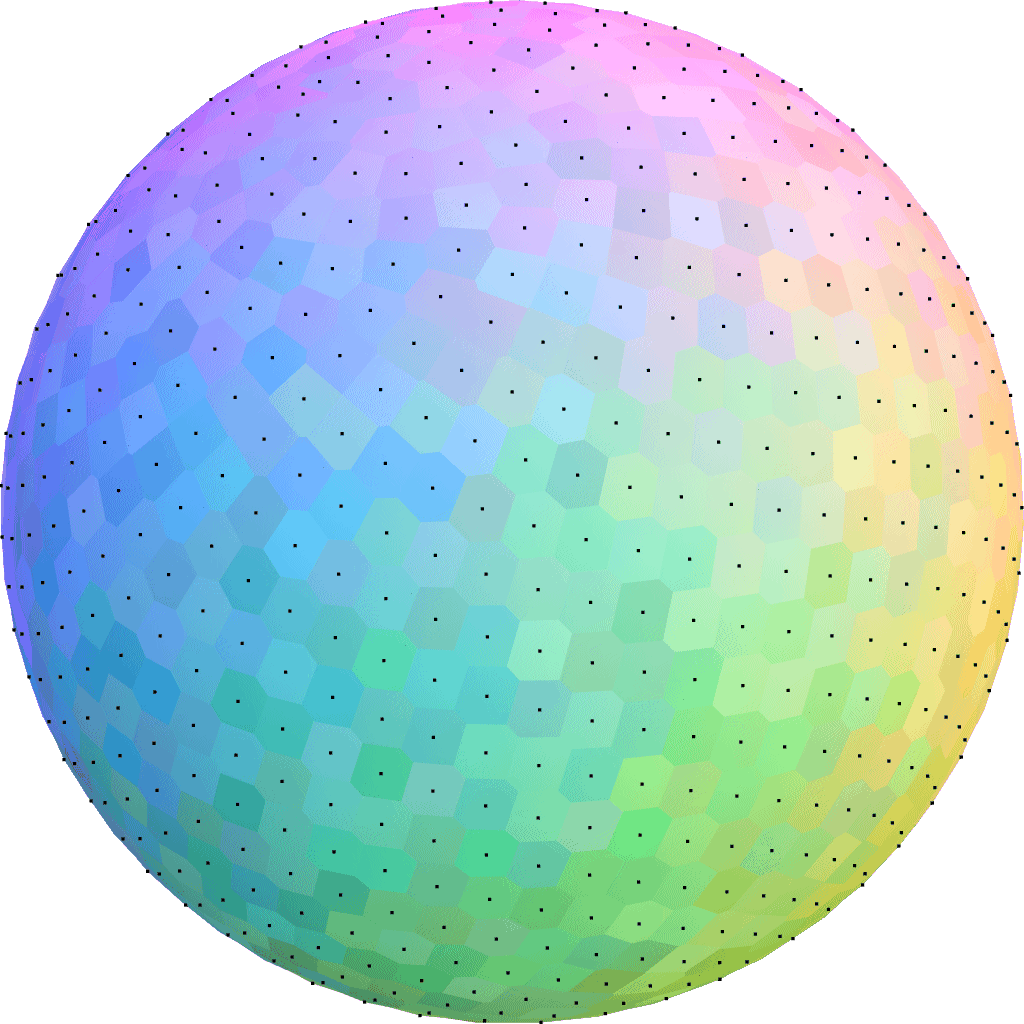
\includegraphics[scale=0.2]{img/sphere/fibonacci-sphere-voronoi.png}
        \caption{Résultat de l'application d'un diagramme de Voronoï sur une sphère.\protect\footnotemark}
        \label{voronoi}
    \end{center}
\end{figure}

\footnotetext{\href{https://www.redblobgames.com/x/1842-delaunay-voronoi-sphere/}{https://www.redblobgames.com, Delaunay + Voronoi on a sphere
Posted on March 10, 2019 by RedBlobGames}}

\newpage
\subsection{Algorithmes de générations procédurales aléatoires}

    Il existe des algorithmes souvent utilisés dans l'industrie du jeu vidéo et de la modélisation 3D permettant de générer procéduralement à partir de textures avec une part d'aléatoire, des environnements plus ou moins réalistes comme des terrains, des nuanceurs ("shader" en anglais), etc. Un exemple est présent sur la figure \ref{figure5}.
    
    \begin{figure}[!h]
        \begin{center} 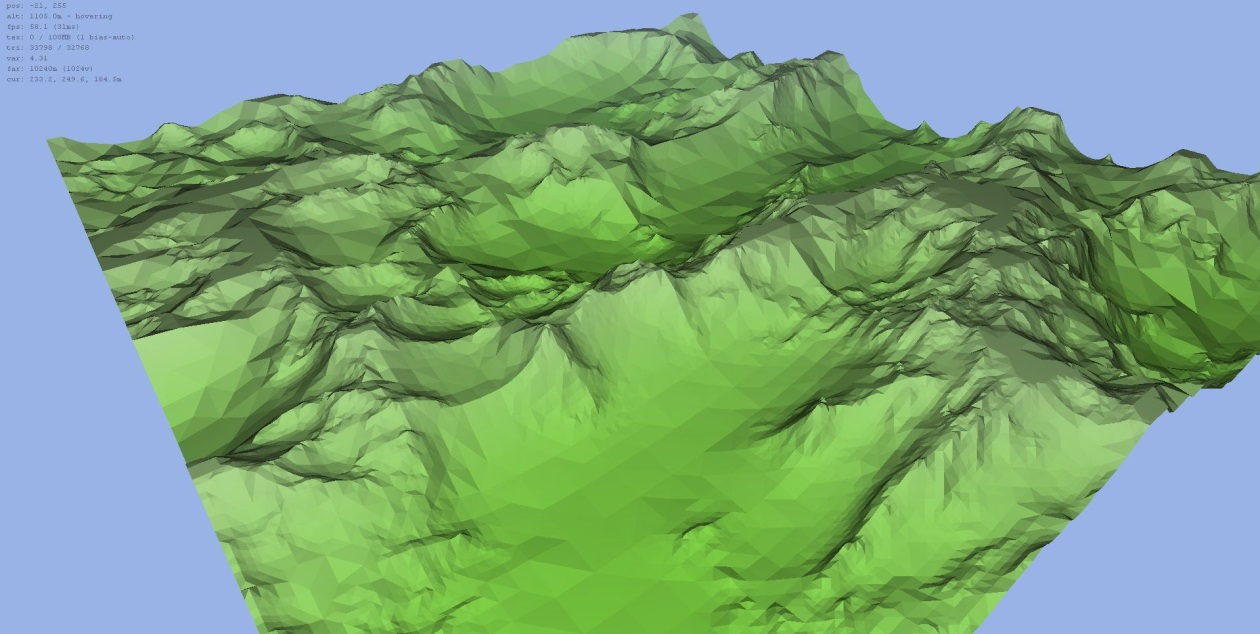
\includegraphics[width=0.8\linewidth]{img/landscape.jpg} \end{center}
        \caption{\label{figure5}Image de terrain généré procéduralement\protect\footnotemark .}
    \end{figure}
            
    \footnotetext{\href{https://sainarayan.me/2015/05/13/procedural-terrain-generation-using-perlin-noise-and-machine-learning/}{https://sainarayan.me, Procedural Terrain Generation
Posted on May 13, 2015 by Cyber Shaman}}
        
    Ces algorithmes se basent sur le modèle du "bruit" mathématique utilisé dans la théorie des signaux, mais avec des paramètres qui permettent de varier les effets. C'est ce qu'on appelle le "chaos", de l'aléatoire contrôlé.\\
    Un exemple très simple serait le bruit dit "blanc"(figure \ref{whitenoise}), ne faisant pas partie de ces bruits chaotiques et est purement aléatoire. Il est peu intéressant pour générer des environnements réalistes, et c'est pour cela que l'on écartera tous les bruits que l'on ne peut pas contrôler.\\
    
        \begin{figure}[!h]
        \begin{center} 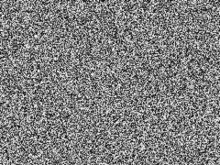
\includegraphics[width=0.4\linewidth]{img/noise/whitenoise.png} \end{center}
        \caption{\label{whitenoise}Image de bruit blanc\protect\footnotemark .}
        \end{figure}
            
        \footnotetext{\href{https://upload.wikimedia.org/wikipedia/commons/thumb/f/f6/White-noise-mv255-240x180.png/220px-White-noise-mv255-240x180.png}{Image from wikipedia}}
        
    Il reste trois types de bruits qui peuvent être intéressant pour ce projet : les bruits de valeurs, les gradients de bruits (Perlin Noise, Simplex Noise), et les bruits organiques (Voronoï, Worley) que l'on peut voir figure  \ref{noises}. Cependant vu la diversité des différents bruits qui existe, le plus intéressant est le bruit de Perlin. Il est le plus utilisé pour réaliser des reliefs de terrain. Il a l'avantage d'être très flexible sur les paramètres donnés, tout en produisant des textures réalistes. Il existe aussi une amélioration moins coûteuse en ressources, Simplex Noise, et qui fait moins d'anormalité sur le rendu 3D (artéfact). Pour plus d'informations, lire \cite{BookShader}.
\newpage
    \begin{figure}[!h]
    \begin{center}
    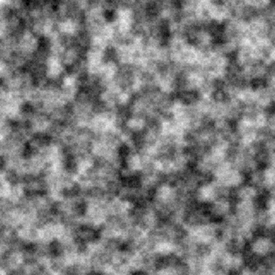
\includegraphics[width=0.4\linewidth]{img/noise/value.png}
    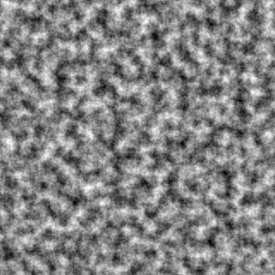
\includegraphics[width=0.4\linewidth]{img/noise/perlin.png}
    \end{center}
    \begin{center}
    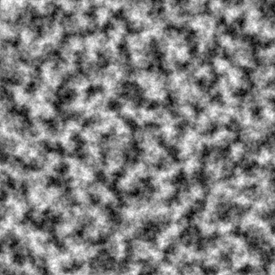
\includegraphics[width=0.4\linewidth]{img/noise/simplex.png}
     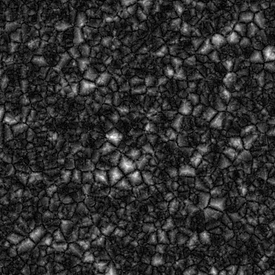
\includegraphics[width=0.4\linewidth]{img/noise/voronoi.png}
     \end{center}
     \begin{center}
    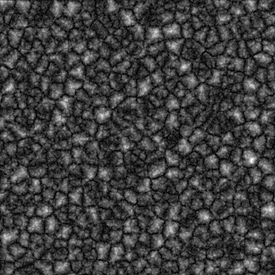
\includegraphics[width=0.4\linewidth]{img/noise/worley.png}
    \end{center}
        \caption{\label{noises}Différents types de bruit\protect\footnotemark.\\
        A partir d'en haut à gauche jusqu'en bas à droite : valeur, Perlin, Simplex, Voronoï, Worley.}
    \end{figure}

    \footnotetext{\href{https://github.com/Scrawk/Procedural-Noise}{Image d'une bibliothèque Github par l'utilisateur Scrawk, Accessed January 2020}}
            
\newpage

\subsection{Rendu graphique 3D} \label{raster/ray}

Il existe deux méthodes principales pour le rendu d'une scène 3D : la rastérisation et le ray tracing.

            La rastérisation est un procédé qui consiste à convertir une image vectorielle en une image matricielle destinée à être affichée sur un écran. On englobe dans la rastérisation tous les procédés permettant d'améliorer l'aspect final du rendu en 3 dimensions.
            Les objets à l'écran sont créés à partir de triangles ou de polygones qui définissent le modèle 3D de l'objet.
            \begin{itemize}
                \item \textbf{Avantages :}
                \begin{itemize}
                    \item Faible coût en mémoire,
                    \item Plus de choix dans la représentation des faces et du modèle (triangles, quadriques, polygones, torres ...),
                    \item La performance dépend directement du nombre de faces.
                \end{itemize}
                \item  \textbf{Inconvénients :}
                \begin{itemize}
                    \item Rendu simplifié non réaliste,
                    \item Ne prend pas en compte les reflets, la transparence, l'effet miroir.
                \end{itemize}
            \end{itemize}
        
Une autre méthode existante est le ray tracing qui remédie aux inconvénients de la rastérisation. Cette technique reproduit les phénomènes physiques que sont la réflexion et la réfraction. Cela permet un rendu plus réaliste en tenant compte de la lumière, des reflets ou encore de la transparence. Cependant, il s'agit d'avantages qui ne correspondent pas aux besoins clients. Il a donc été décidé de ne pas se pencher sur cette technique de rendu et d'utiliser la rastérisation.
        
\subsection{Outils existants et prototypes}

\subsubsection{Blender \cite{Blender}}

Afin de pouvoir générer et afficher la planète, une des solutions qui peut-être abordée est l'utilisation d'outils de modélisation en 3 dimensions. Ils disposent déjà de moteurs de rendu performant, dont certains utilisent un système de scripting et de plugin afin de générer des formes, les modifier, et les texturer, pour ensuite les utiliser plus tard dans d'autres logiciels, selon des formats standardisés.

L'un de ces outils existant est l'outil Blender. Il est tout d'abord un logiciel open source, dont le moteur interne est en C/C++ permettant de bonnes performances. Il dispose aussi d'une API en Python permettant un prototypage très rapide.

Un script python a été écrit permettant de :
\begin{enumerate}
            \item {créer une icosphère d'environ 10 000 polygones}
            \item {appliquer une transformation sur ses sommets selon une texture de Voronoï.}
            \item {afficher les paramètres et le temps de génération.}
\end{enumerate}

Le script est disponible dans la hiérarchie du projet \textit{docs/requirements/test\_blender} ainsi que les résultats. Le premier résultat obtenu en exportant l'image depuis l'éditeur est visible sur la figure \ref{blendericos}.\\

\begin{figure}[!h]
\begin{center} 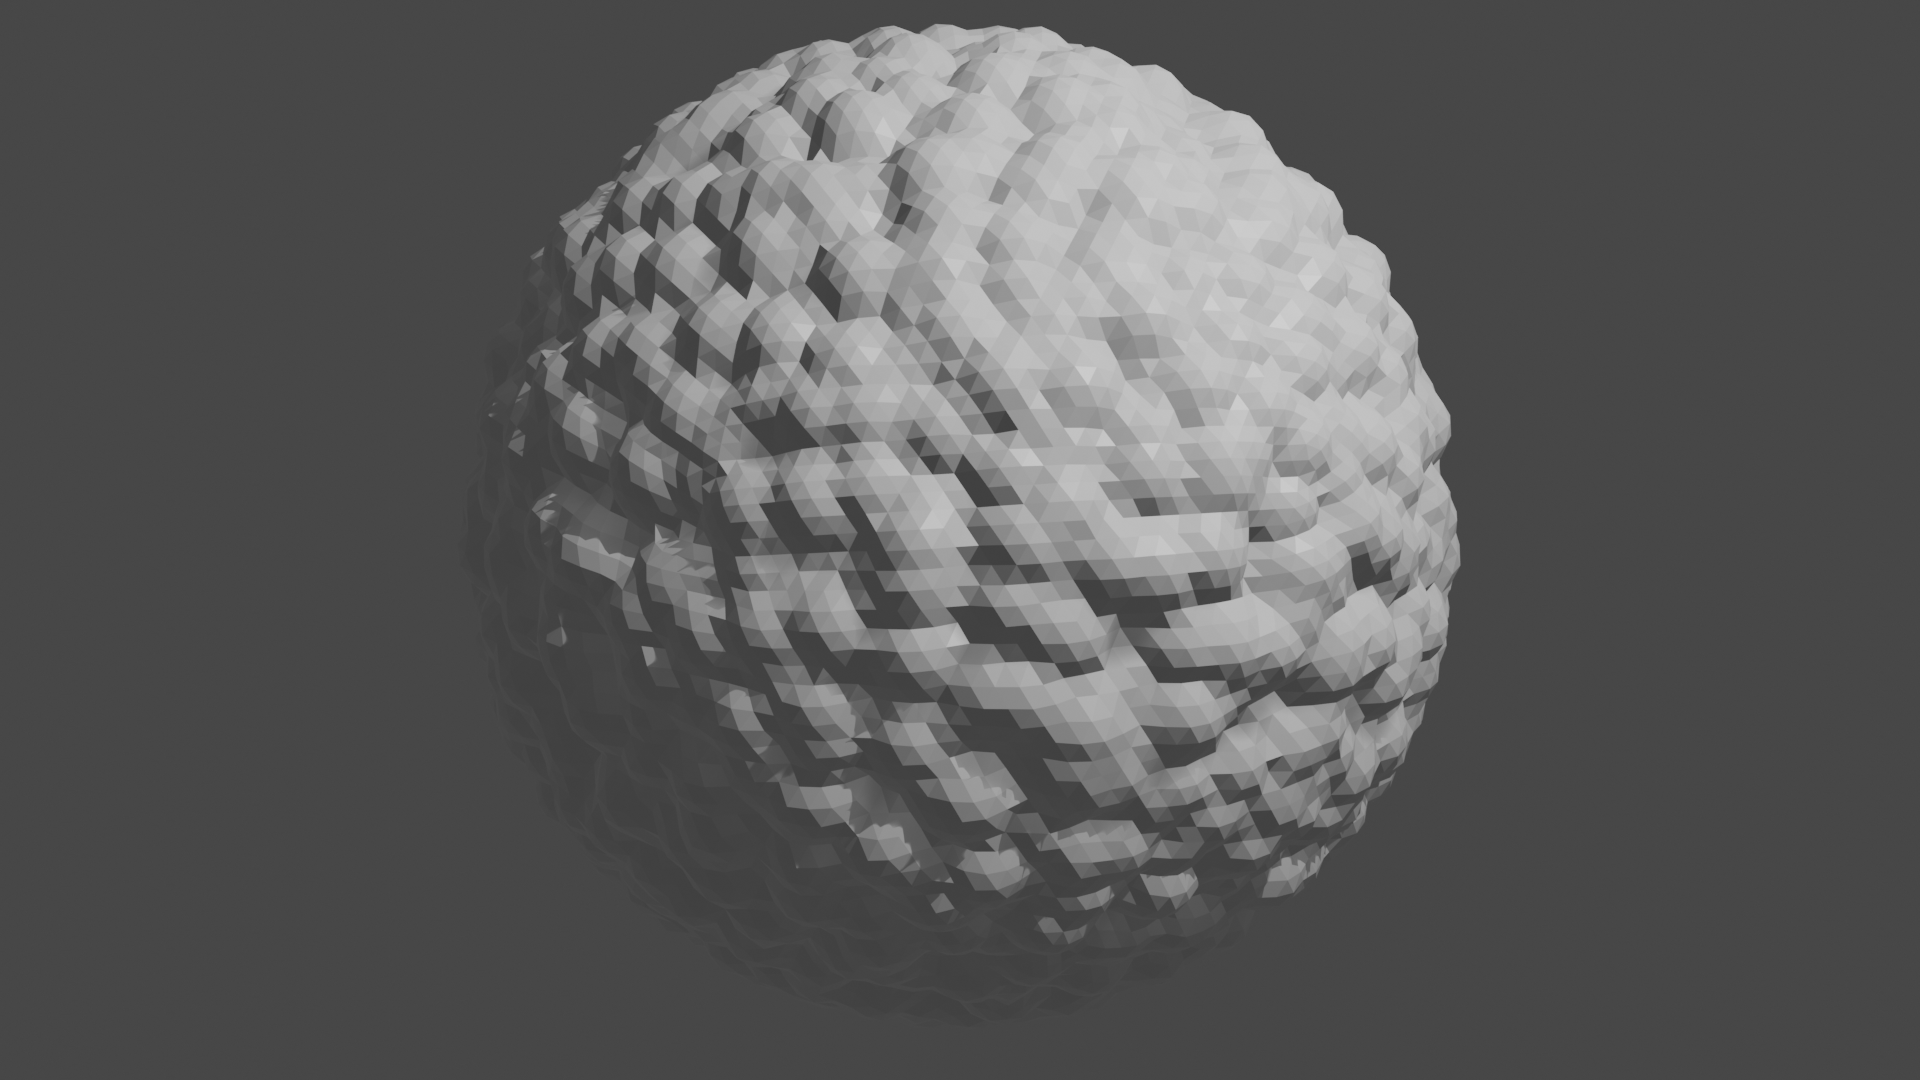
\includegraphics[width=0.8\linewidth]{img/blender/blender_1.png} \end{center}
\caption{\label{blendericos}Icosphère générée par Blender. Texture de bruit Voronoï, 6 subdivisions, \textasciitilde0.02 s, 20480 polygones}
\end{figure}

Attention à la version de Blender. Le moteur de rendu utilisé est Evee version 2.8 permettant une visualisation sans dégradation lors du déplacement de point de vue (rotation, zoom) avec les rendus finaux. Pour des soucis de performance, il faut aussi faire attention à la machine utilisée, notamment la carte graphique.\\

Les paramètres ont été changés depuis l'éditeur Blender afin d'arriver aux résultats figure \ref{blendericosmodif} et \ref{blendericosmodifedit}.\\

\begin{figure}[!h]
\begin{center} 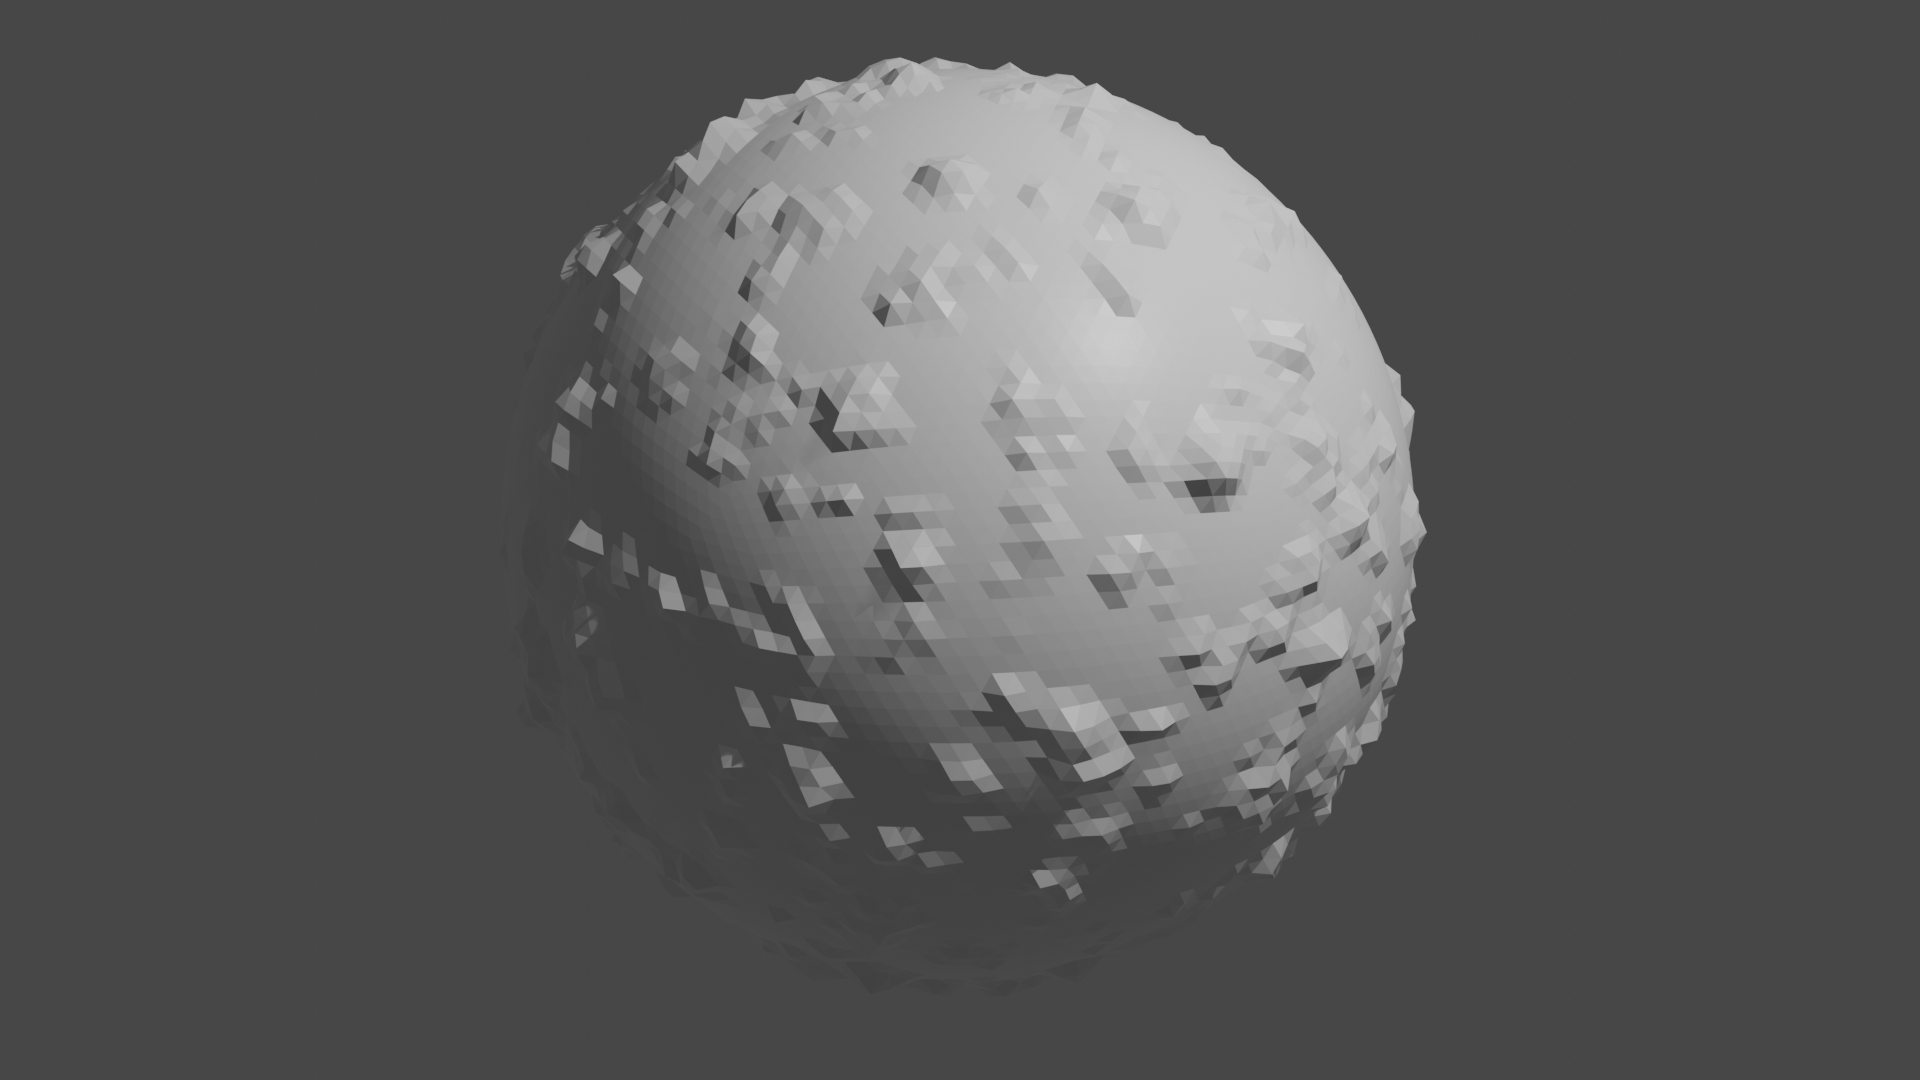
\includegraphics[width=0.8\linewidth]{img/blender/blender_2.png} \end{center}
\caption{\label{blendericosmodif}Modification de la texture de bruit Voronoï sans couleur}
\end{figure}

\begin{figure}[!h]
\begin{center}
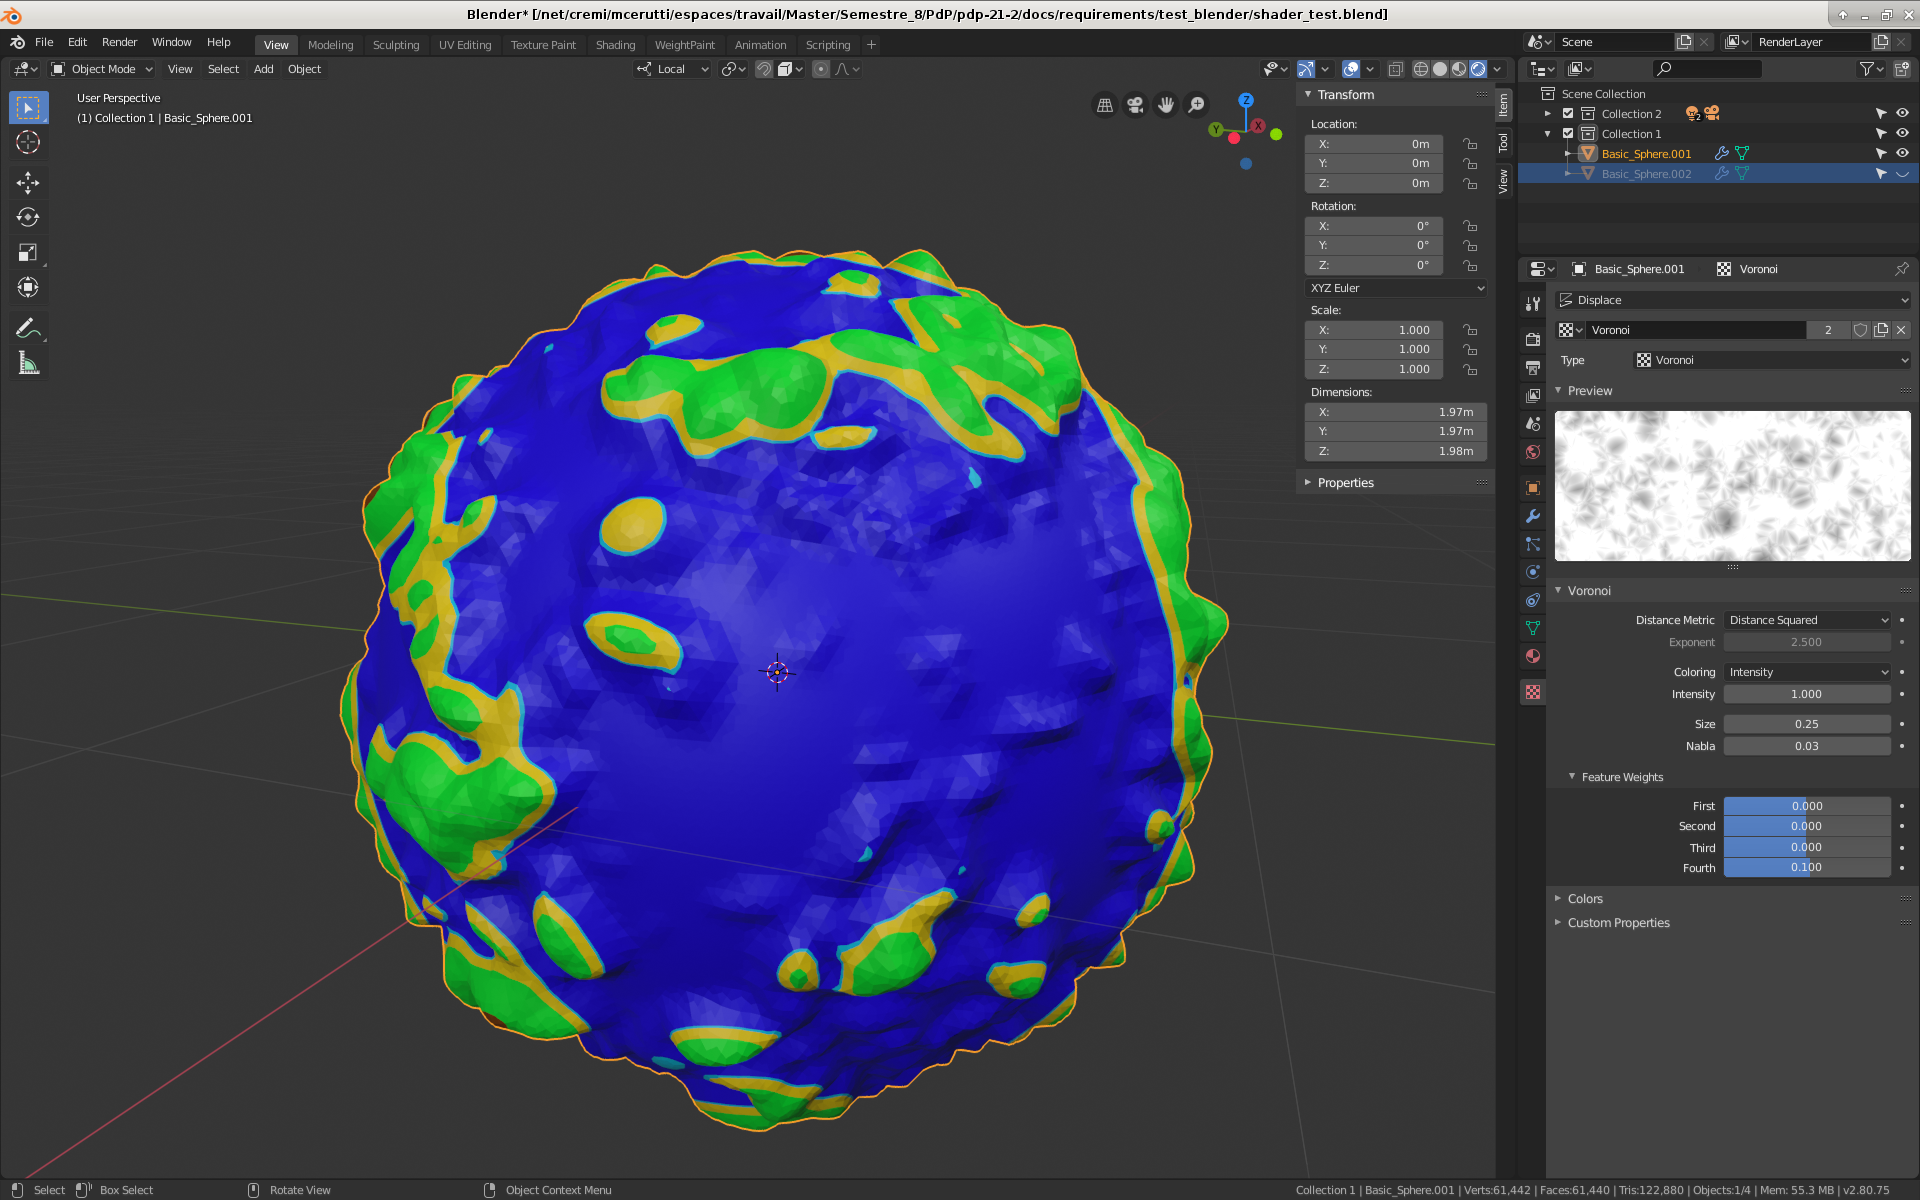
\includegraphics[width=0.8\linewidth]{img/blender/blender_editeur_bruit.png}
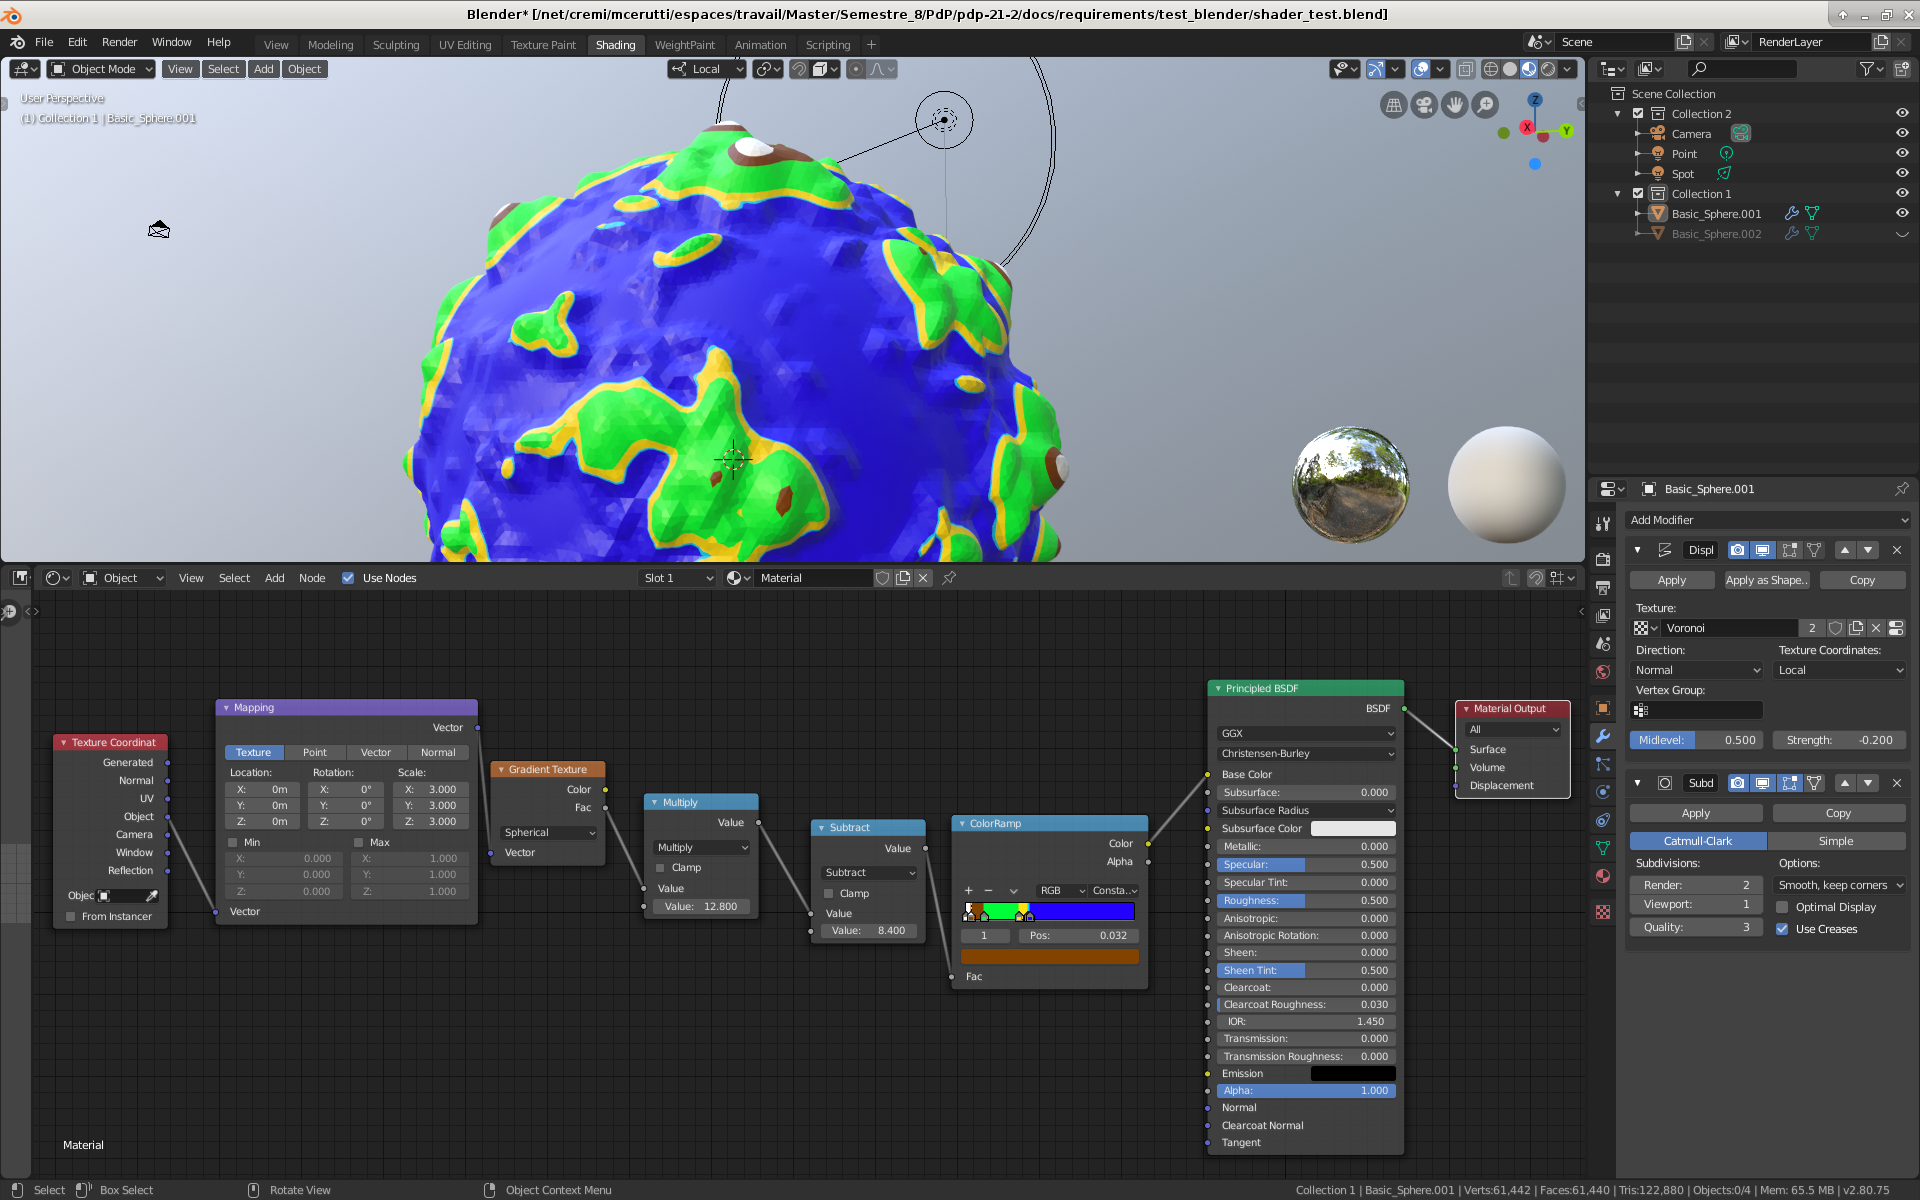
\includegraphics[width=0.8\linewidth]{img/blender/blender_shaderEditor.png}
\end{center}
\caption{\label{blendericosmodifedit}Essais de modifications par l'éditeur Blender : paramètres de texture, bruit de déplacement des sommets, rajout de nuances (shader)}
\end{figure}

\newpage
\paragraph{Avantages}

\begin{enumerate}
            \item {Rendu de base avec OpenGL, Moteur interne en C/C++ :}
            Permet d'espérer de très bonnes performances au niveau des algorithmes de base. Crucial dans le cas de rendu de l'ordre de 60 images par secondes (FPS) avec une bonne machine.
            
            \item {Open source et sous GNU General Public License (ou "logiciel libre") :}
            Cela permettrait de modifier le moteur de rendu, et les algorithmes de visualisation selon les besoins.
            
            \item {Multi-plateforme :}
            Permet le portage Linux (correspondant à notre besoin), et aussi sur d'autres plateformes nativement.
            
            \item {API très simple en Python afin d'accéder et de modifier la forme :}
            Permet de faire des tests très rapides, et de laisser le client manipuler les algorithmes de modification plus facilement qu'on aurait implémenté en sur-couche du moteur interne.
            
            \item {Fonctionnalités supplémentaires (sauvegarde, modification, amélioration de rendu, création de nuauceurs en noeuds...) :}
            Permettrait de se focaliser davantage sur les fonctionnalités concernant la génération de la planète, en ayant déjà les possibilités d'extensions de notre projet.
            
\end{enumerate}

\paragraph{Inconvénients}

    \begin{enumerate}
                
                \item {Ne convient pas à l'exercice du PDP :}
                étant informaticiens et non des graphistes, il n'y a aucun intérêt pédagogique à utiliser un outil aussi complet. Son utilisation nécessiterait aucunement une équipe de 5 personnes, et encore moins au sein d'une formation informatique.
                
                \item {Interface de Blender trop riche pour le client :}
                contraire à la demande du client demandant une visualisation simple. Nécessite une connaissance au moins de surface de l'outil. Risque de refus à envisager avant de commencer à l'utiliser.
                
                \item {La version de Blender influe sur l'API (la version 2.8 n'est pas encore formellement documentée), et sur les performances de rendu (moteur Evee) :}
                risques d'instabilité et de bug sur l'API fournie, ainsi qu'un développement plus chaotique du fait d'un manque de documentation.
                
                \item {Pas de sécurité sur des paramètres trop grands (cesse de fonctionner, pas d'erreurs de ressources si demande trop grande) :}
                lié au fait d'utiliser une API en "boîte noire", nécessite un apprentissage des fonctions du moteur interne et une bonne documentation. Cela aussi influe sur la flexibilité du code et les limites d'extensions avec le logiciel de base.
                
                \item {Rendu et génération dépendant de la machine choisi :}
                il est nécessaire d'avoir une configuration suffisamment puissante pour pouvoir utiliser cet outil (se référer à la configuration du client \ref{Compatibilité}).
                
    \end{enumerate}
    
\subsubsection{OpenGL}
\label{choixoutil}
OpenGL (Open Graphics Library) est considérée comme une API (Application programming interface) qui offre la capacité d'afficher des objets en 2D et en 3D. Elle est principalement utilisée pour interagir facilement avec les cartes graphiques (GPU). Elle est utilisée en C/C++. Néanmoins, c'est avant tout une spécification, qui décrit ce que sont les entrées et sorties de chaque fonction et comment elles doivent s'exécuter. Cette spécification est implémentée par les constructeurs de carte graphique (dans les pilotes). OpenGL est disponible sous plusieurs versions.
La version 3.3 quant à elle, est une base de la programmation moderne d'OpenGL (et donc actuellement la plus utilisée) et permet une grande flexibilité et efficacité. Qui plus est, les versions supérieures à celle-ci implémentent des fonctionnalités supplémentaires sans changer les précédentes. Il y a donc un faible problème de compatibilité. Il est tout à fait possible d'afficher une sphère de plus de 10 000 polygones, comme le prouve la figure \ref{sphereOpenGL}.


\begin{figure}[!h]
\begin{center}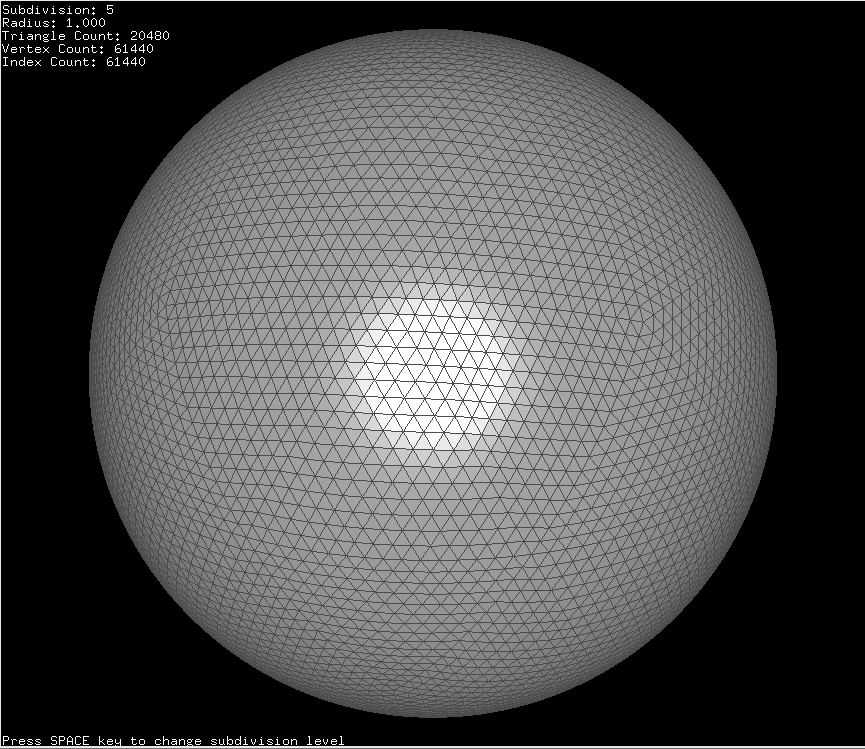
\includegraphics[width=0.6\linewidth]{img/icosphere.png} \end{center}
\caption{Affichage d'une sphère en OpenGL avec plus de 10000 polygones}
\label{sphereOpenGL}
\end{figure}

\paragraph{Avantages}
    \begin{enumerate}
                \item {Performant :}
                Ces bibliothèques sont implémentées en C/C++ et sont utilisées par de nombreuses compagnies, studios et équipes de développement afin de faire des applications graphiques performantes (60 images par secondes et définition 4K maintenant). On peut donc espérer avoir de bonnes performances concernant le logiciel.
                
                \item {Accessible :}
                Les principales bibliothèques dérivées d'OpenGL ont une bonne documentation et de nombreux tutoriels. Cela permet d'avoir plus de temps pour l'implémentation sachant que l'apprentissage sera plus aisé.
                
    \end{enumerate}

\paragraph{Inconvénient}
    \begin{enumerate}
                \item {Temps de développement :}
                Du fait que OpenGL est en C/C++, la réfléxion pour la gestion mémoire et l'architecture demandera du temps. Il sera donc nécessaire d'avoir ces faits en tête lors du développement.
                
                \item {Complexité de prise en main :} 
                OpenGL et ses bibliothèques offrent une très grande flexibilité mais la compréhension et la prise en main de celles-ci est très complexe, comme il y en a beaucoup. Même avec les bons tutoriels et une bonne documentation, il faudra prendre en compte l'apprentissage dans le temps passé au développement.
                
    \end{enumerate}
    

\subsubsection{Gestion de fenêtre et interaction utilisateur}
    OpenGL ne permet pas directement de gérer des fenêtres et des évènements d'entrée (clavier/souris). En revanche, il existe principalement deux bibliothèques open source qui étendent OpenGL et permettent cela : freeglut\cite{freeglut} (écrit en C et sous licence X-Consortium) et GLFW\cite{GLFW} (écrit en C et sous licence zlib/libpng).\\
    
    Ces bibliothèques mettent des fonctions à disposition dont la création de fenêtre en indiquant ses dimensions. Il faut ensuite utiliser une boucle de rendu pour garder la fenêtre ouverte, continuer de dessiner les images et gérer les entrées utilisateur.\\
    
    Il n'y a pas vraiment de différence de fonctionnalité entre ces deux bibliothèques, si ce n'est que freeglut est basé et étend la bibliothèque GLUT qui était très utilisé par le passé mais sous droit d'auteur privé et dépassé.
 
 \subsubsection{Moteurs de jeux}

    Il est possible de s'intéresser aux moteurs de jeux. Le seul moteur de jeu qui aurait pu être intéressant est Godot, car il est open source et est sous licence MIT qui a des avantages au niveau de la distribution et de son utilisation comparé aux concurrents les plus utilisé Unity et Unreal Engine. Mais cette solution a été vite écartée pour trois grandes raisons : 
    \begin{enumerate}
        \item  La première est que les moteurs de jeux, bien qu'ils aient un moteur de rendu 3D intégré sont beaucoup trop fournis en fonctionnalités. La plupart des fonctionnalités ne sont pas intéressantes pour ce projet. 
        
        \item La deuxième est que cela ne convient pas à l'exercice du PDP, en soit faire une sur-couche et faire quelques modifications aurait suffi, mais ce n'est pas le but pédagogique de PDP.
        
        \item  La dernière est que bien que le moteur de rendu permet d'avoir déjà des optimisations, il risque d'y avoir encore plus de code qui peut ralentir le rendu. Pire, cela rajoute des dépendances et l'installation d'un moteur de jeu par le client, ce qui est contraire à une interface simple.
    \end{enumerate}

\newpage
\section{Besoins fonctionnels}


Le comportement d'utilisation du logiciel est décrit sur la figure \ref{diagrammeflux}. Ce comportement ce traduit par les différents besoins fonctionnels et non fonctionnels évoqués ci-dessous.
\begin{figure}[!h]
\begin{center}\includegraphics[scale=0.3]{img/diagramme_de_flux.png} \end{center}
\caption{Diagramme de flux du logiciel de génération et de visualisation de planète}
\label{diagrammeflux}
\end{figure}

\subsection{Créer un espace 3D}
            Afin d'être cohérent tant au niveau de la génération que de la visualisation, il faut d'abord définir un espace 3D commun aux deux, et donc définir le repère, et l'échelle.
            
            \subsubsection {Choix du repère :}
            Du point de vue de l'implémentation du repère, la bibliothèque de départ et son propre système de coordonnées sera un facteur important quant au choix de l'abstraction, mais en soit il existe deux possibilités (figure \ref{reperes}) :
            \begin{itemize}
                \item Un repère orthonormé.
                \item Un repère angulaire.
            \end{itemize}
            
            \begin{figure}[!h]
            \begin{center}
            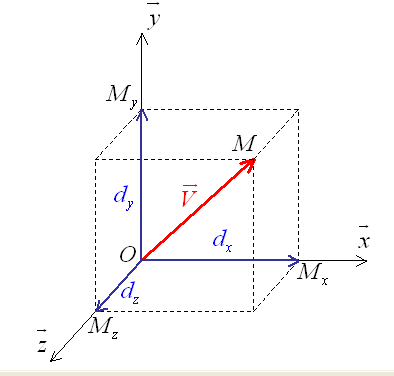
\includegraphics[width=0.4\linewidth]{img/rep_ortho.png}
            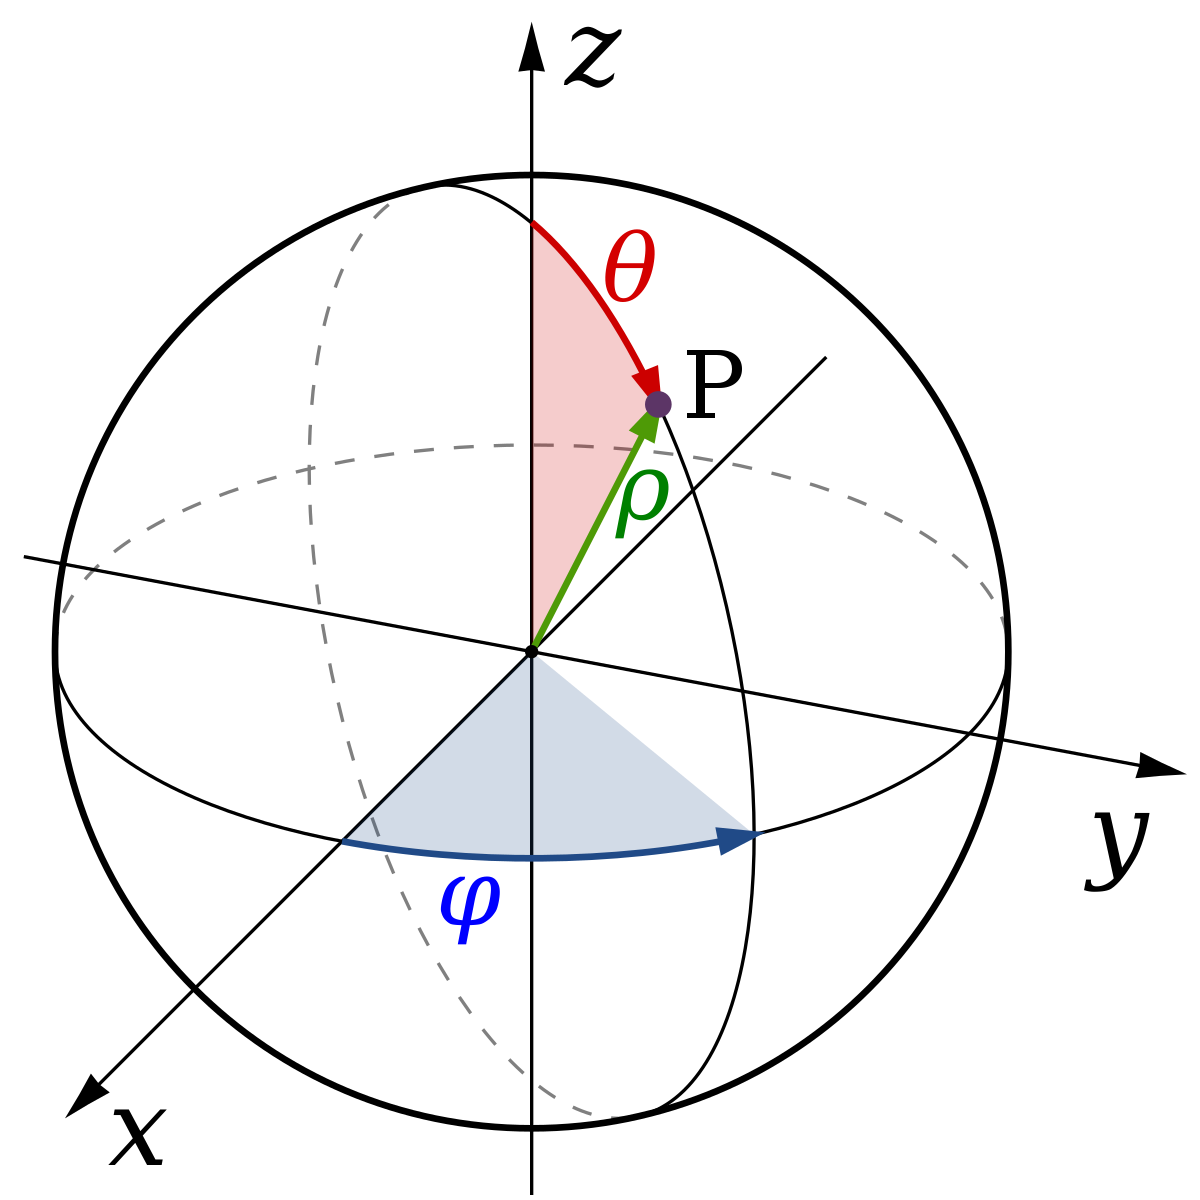
\includegraphics[width=0.3\linewidth]{img/rep_sphere.png}
            \caption{Repère orthonormé \protect\footnotemark et repère angulaire \protect\footnotemark}
            \label{reperes}
            \end{center}
            \end{figure}

            \footnotetext{\href{https://www.wikimeca.org/index.php/Outils_math\%C3\%A9matiques:Vecteurs}{Wikipedia  Outils mathématiques:Vecteurs, Accessed January 2020}}
            \footnotetext{\href{https://fr.wikipedia.org/wiki/Coordonn\%C3\%A9es_sph\%C3\%A9riques}{Wikipedia Coordonnées sphériques, Accessed January 2020}}
            
            Pour le repère orthonormé, on peut faciliter les calculs et la représentation en utilisant comme origine du repère le centre de la planète, n'ayant pas d'autres objets à représenter sur la scène.\\
            Ce système a comme avantage d'être simple à implémenter, et d'être relativement intuitif sur la visualisation pour le débogage.\\
            L'autre possibilité serait de raisonner selon des coordonnées sphériques, et une hauteur de sommet par rapport au centre de la sphère, en utilisant un repère angulaire couplé à une altitude. Cela a l'avantage de faciliter les calculs en cas d'application des textures, de génération des positons des sommets, et aussi de raisonner selon un système physique de longitude et latitude. On préférera cette approche. \\
            \\
             Cependant il y a très peu d'outils qui utilisent des coordonnées radiales. Il faudra sûrement combiner les deux systèmes.\\
            
            \subsubsection {Choix de l'échelle :}
            
            Il faut aussi fixer une unité de mesure pour la distance entre les sommets de la surface et le centre de la planète, afin de mieux pouvoir appréhender les valeurs de hauteur fixées des sommets (figure \ref{echelle}).\\
            
            \begin{figure}[!h]
            \begin{center}
            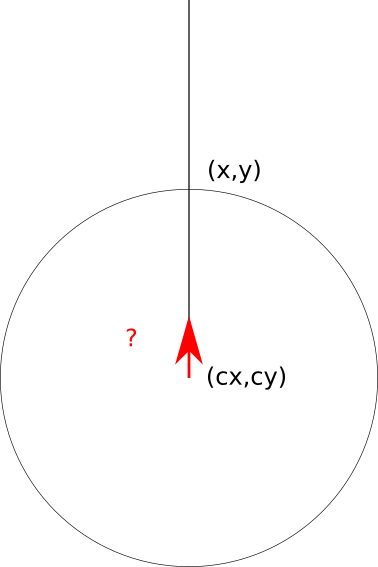
\includegraphics[width=0.2\linewidth]{img/echelle.png}
            \caption{Échelle représentation}
            \label{echelle}
            \end{center}
            \end{figure}
            
            Une possibilité pour ça est de choisir un niveau fixe, comme un niveau de la mer qui serait une sphère parfaite et de raisonner à partir de celui-ci. Pour faciliter le code, on pourrait ramener l'altitude entre l'espace [-1,1], 0 étant le niveau de la mer, -1 étant l'altitude du centre de la terre. Les valeurs de la hauteur se retrouvent donc bornées.\\
            
            Une autre façon est de ne pas faire de niveau de mer et de laisser les valeurs à partir d'une unité arbitraire. Avec ce système, il suffit de multiplier l'unité par une valeur physique pour pouvoir représenter des valeurs comparables à la réalité. On préférera ce système pour faciliter les calculs, et parce qu'il présente comme avantage, par rapport au premier de raisonner qu'avec des valeurs positives, qu'on peut associer à une représentation réaliste.\\
            
            
\subsection{Génération procédurale d'une planète}
    
    Maintenant que nous avons notre espace défini, il nous faut choisir quelle géométrie nous allons adopter pour la sphère. Elle va influencer le parcours et la construction de celle-ci.
    
    Il faut ensuite définir quelles informations utilisées pour la génération de la planète, et lesquelles semble faisable et pertinent pour ce projet.\\
    
    Cela conduit au traitement décrit figure \ref{sequence}. 

    \begin{figure}[!h]
            \begin{center}
            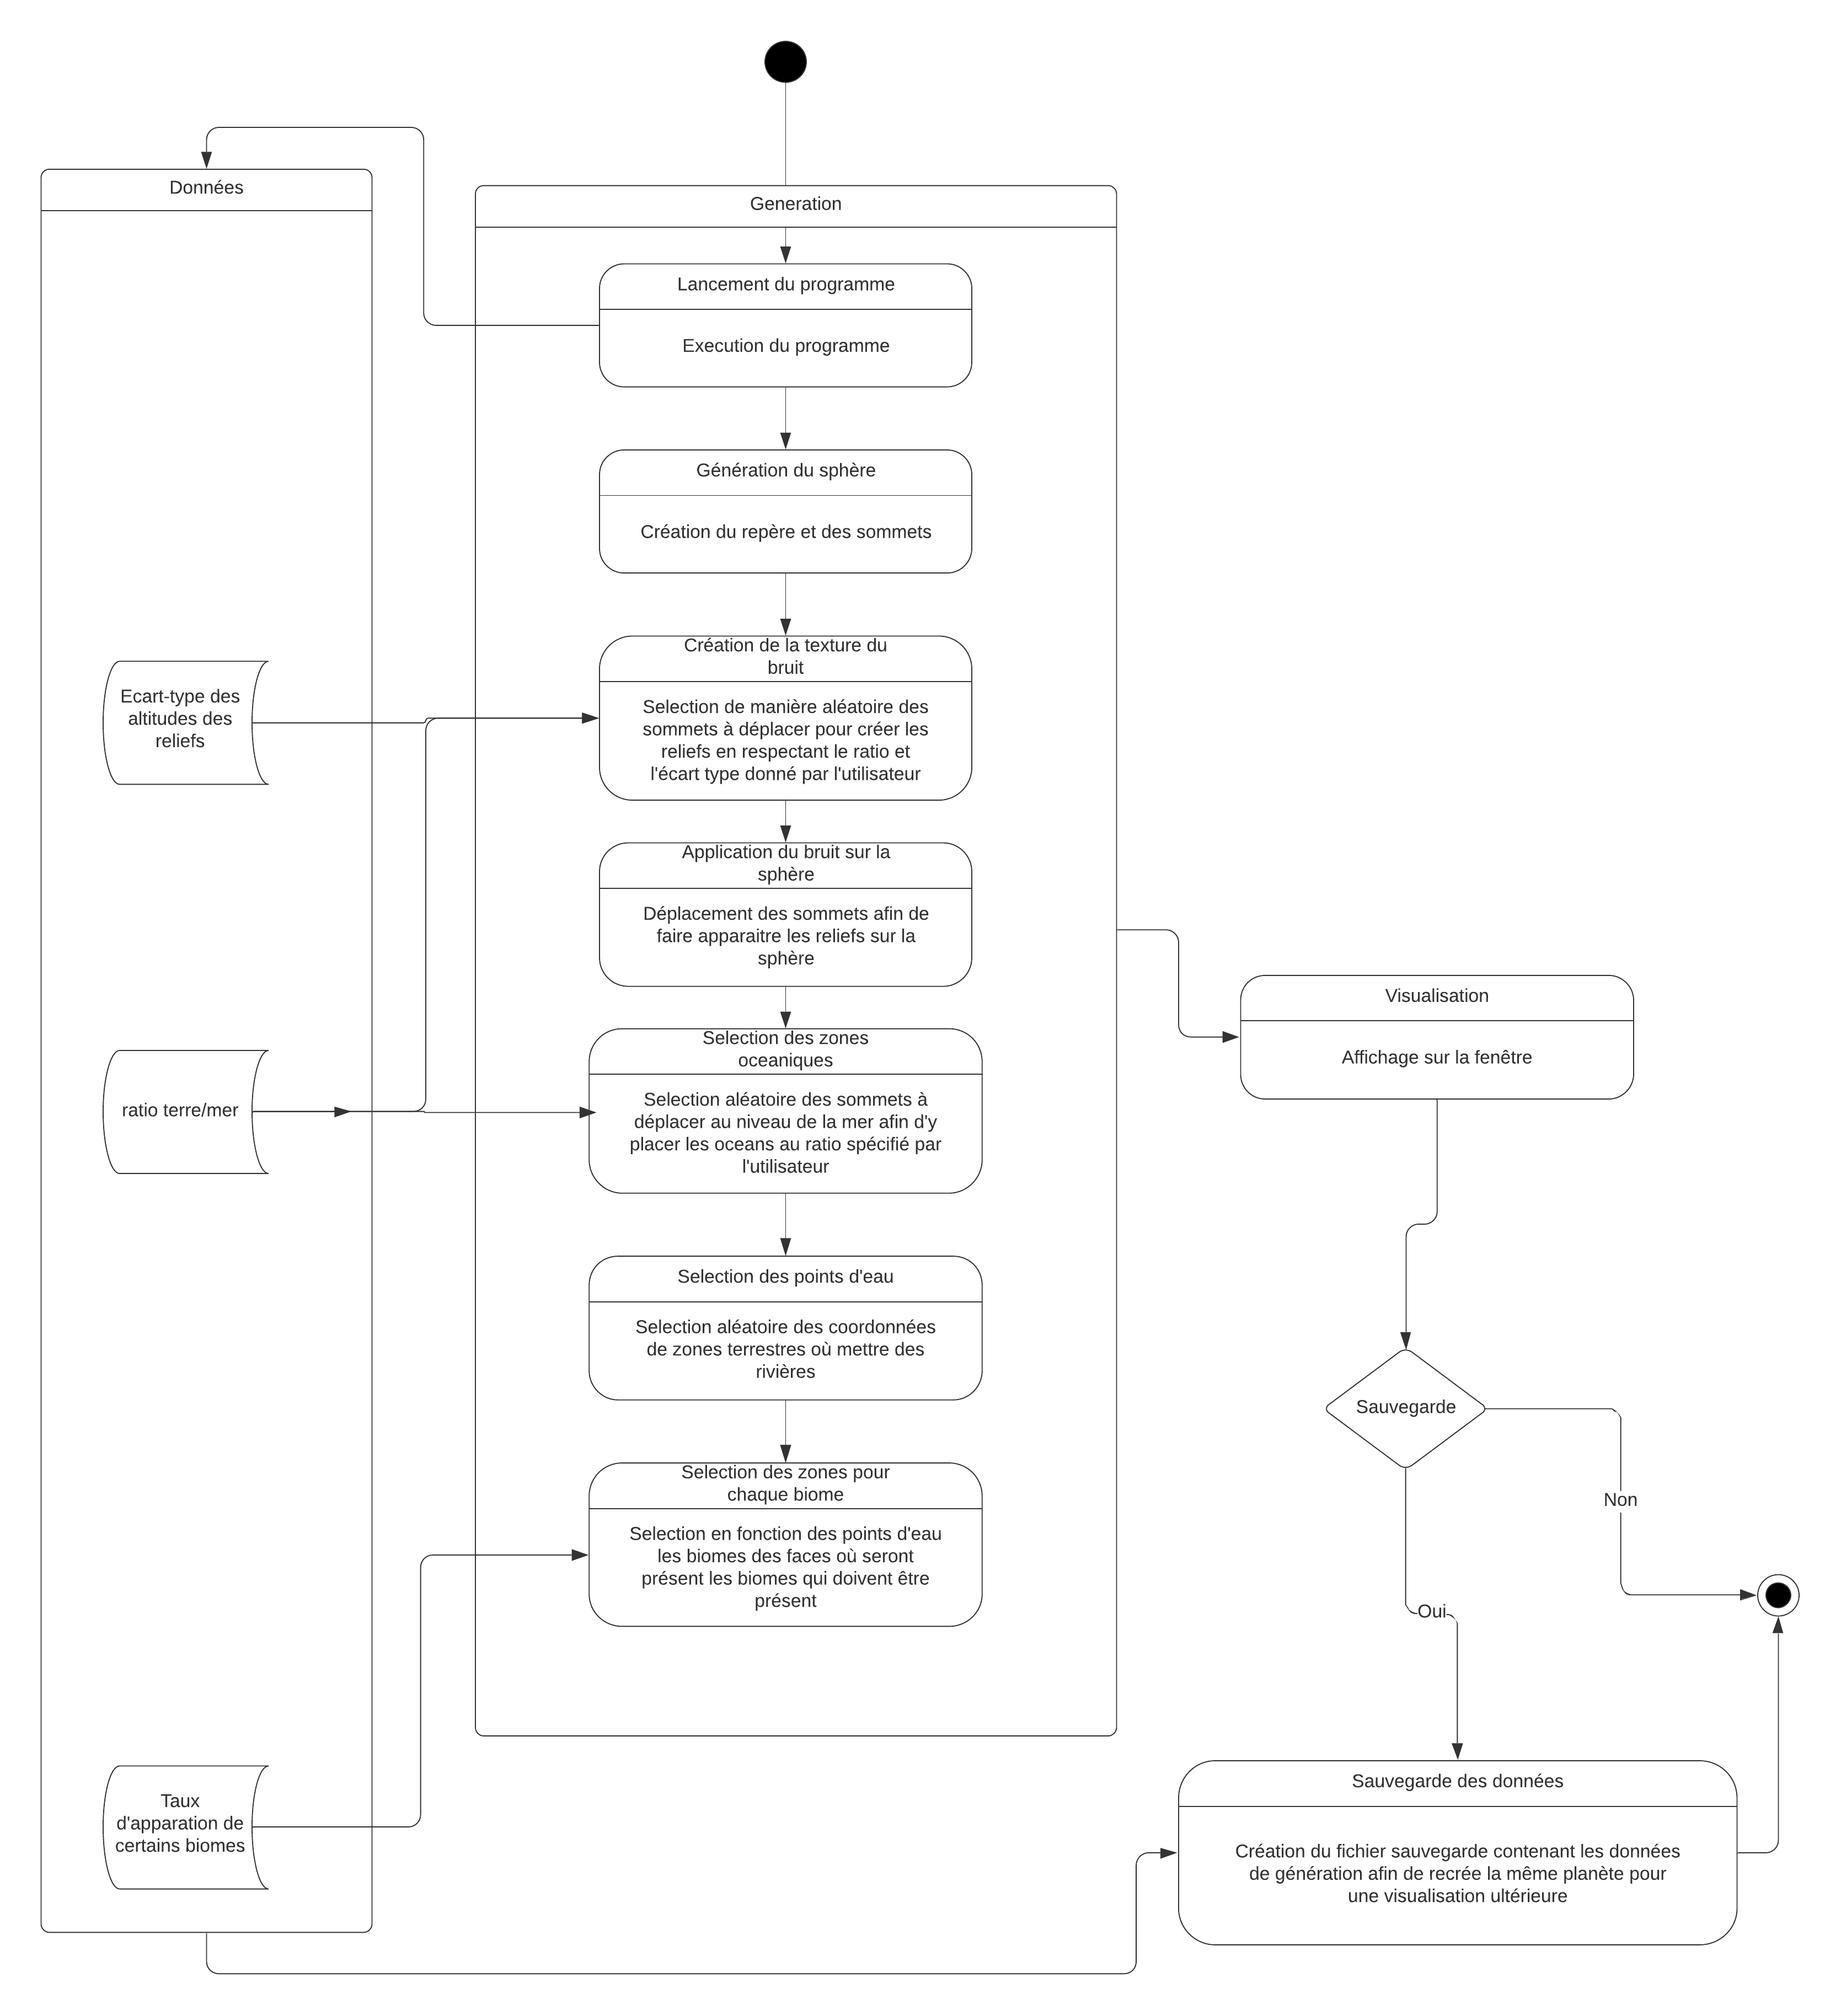
\includegraphics[scale=0.6]{img/workflow_chart.png}
            \caption{Diagramme séquentiel de la génération et visualisation d'une planète.}
            \label{sequence}
            \end{center}
    \end{figure}
    \newpage
    \subsubsection{Créer la géométrie}

    La planète est caractérisée par une sphère. Il doit donc être nécessaire de pouvoir créer une sphère. L'analyse de l'existant à montrer qu'il existait plusieurs techniques avec deux approches de départ différentes : avec des points, ou directement avec des formes.  La solution la plus adéquat est l'utilisation de l'icosaèdre avec sa subdivision. C'est une méthode tout à fait standard et efficace qui ne nécessitera pas l'implémentation d'algorithmes supplémentaires pour un rendu minimal correct à l'inverse de la sphère de Fibonnaci. Qui plus est, l'implémentation et l'utilisation d'algorithmes supplémentaires pour améliorer le rendu est tout à fait envisageable avec l'utilisation de l'icosaèdre. L'extensibilité  est donc permise avec son utilisation.
                
    \subsubsection{Générer les informations de la planète}
    
            La géométrie définit précédemment, en soit une sphère quasi-parfaite, servira de forme de base à notre planète. Ce n'est qu'après qu'on peut la modifier à notre guise. Ce qui amène du coup à la définition même des informations que l'on va créer et représenter, et dans quelle mesure l'utilisateur peut l'influencer.
    
            \paragraph{Paramètres de la génération.}
            Il doit être possible pour l'utilisateur de guider la génération d'une planète en passant des paramètres à l' algorithme/générateur. Ce passage de paramètres pourrait simplement se faire par ligne de commande lors de l'appel à l'exécutable. Ces paramètres influeront donc sur les transformations appliquées à la planète (plus ou moins d'altitude, de type de terrain... Par exemple, \verb|./planet -altitude 5| , accentuerai d'un facteur 5 la présence de montagnes).
            
            On pourra dans un deuxième temps faire un fichier de configuration en XML et utiliser un parseur, si on veut faire des paramètres plus complexe à notre algorithme.
    
            \paragraph{Rajouter de l'aléatoire.}
            Afin de simplifier les paramètres à donner, et pour faire varier les résultats de génération, il a été choisi de  rajouter de l'aléatoire. Il serait généré grâce à des algorithmes de "bruit" (généré procéduralement), qu'on projette sur la surface de la planète. Celui retenu dans un premier temps sera le bruit appelé "Simplex"(voir \cite{BookShader}).
            
            \paragraph{Liens entre les différentes informations.}
            La combinaison de ces informations  comme l'altitude des sommets, la couleur, etc, se fera sous forme de "couches" superposables, et liées les unes aux autres (par exemple des villes qui sont au dessus d'une certaine hauteur, de l'eau, etc). \\
            Pour cela, il  sera possible d'adopter une structure de code séquentiel en fonction des dépendances des couches entre elles. On pourrait tout à fait envisager d'utiliser une structure de graphe pour y parvenir.\\
            
            \paragraph{Information et représentation.}
            Les informations et leur représentation retenues pour ce projet sont définies par ordre de priorité :
            \begin{enumerate}
                \item {Relief} \\
                    Comme dit dans le choix de l'échelle, il s'agit d'un nombre décimale compris entre 1 et -1 représentant le déplacement d'un sommet afin d'avoir une altitude. Pour les hauteurs supérieurs au niveau de la mer, les couleurs à attribuer aux faces seront vert pour les plaines, marron pour les montagnes et blanc pour les pics de montagnes. 
                \item {Mers et océans} \\
                    Toujours par rapport au choix d'échelle, le niveau de la mer sera à 0 par défaut. Toutes les faces avec une altitude inférieure à ce niveau prendront des nuances de bleu en fonction de leur profondeur.
                \item {Rivières} \\
                    Les rivières peuvent être représentées par un chemin allant d'un sommet source vers une mer. Le chemin en question doit se confondre à la mer seulement à son sommet de destination. Le chemin sera représenté par des faces coloriées en bleues en zone terrestre.
                \item {Biomes} \\
                    Il s'agit d'un groupe de faces à approximativement la même altitude, à laquelle il faut changer la couleur et/ou appliquer une texture (forêt, désert ...).
                \item {Plaques tectoniques} \\
                    Les plaques tectoniques seront représentées par des grands groupes de faces, on pourra ajouter des informations concernant les interactions entre les plaques (par exemple, une présence de montagnes sur une zone de subduction). 
            \end{enumerate}
            
\subsection{Visualisation de la planète}

        Maintenant que nous avons défini la planète et ses informations à afficher, nous pouvons aborder sa visualisation. On utilisera la rastérisation comme méthode de rendu car elle convient mieux aux attentes du client que le ray tracing (voir partie \ref{raster/ray}).

        \subsubsection{Afficher la planète} 
        
        Une seule planète doit être affichée à la fois. Afin d'y parvenir, il faut donc créer une fenêtre (éventuellement extensible) qui se lancera lors de l'appel à l'exécutable par ligne de commandes (\verb|./planet| par exemple). Étant donné la visée ludique de cet outil, une fenêtre carrée ou rectangulaire avec seulement la planète au centre semble être le plus approprié pour l'immersion et l'interaction avec la souris (voir figure \ref{itf_souris}, de préférence directement avec l'objet ce qui est plus ludique que l'utilisation de seekbar, voir figure \ref{itf_seekbar}). Pour ce faire, nous préférerons la bibliothèque open source GLFW qui permet de gérer une fenêtre, un contexte, des évènements clavier/souris etc.\\
  
         \begin{figure}[!h]
        \begin{center} 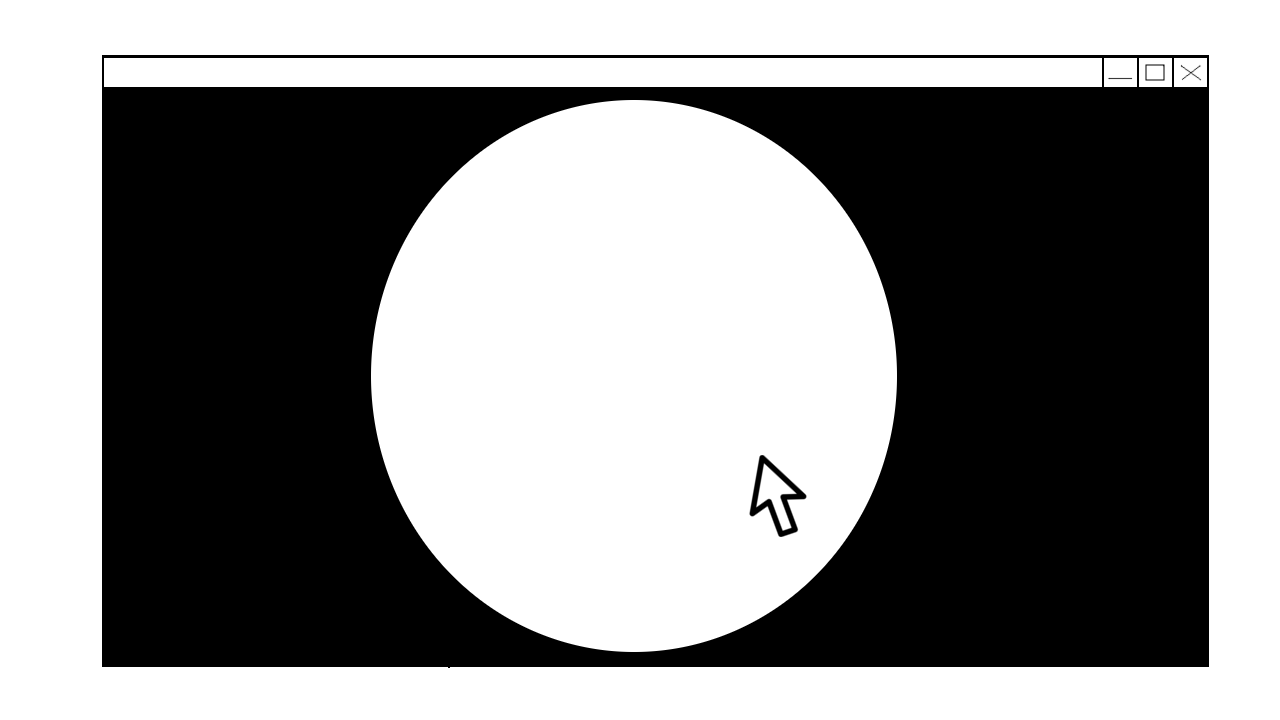
\includegraphics[width=\linewidth]{img/interface_souris.png} \end{center}
        \caption{\label{itf_souris} Prototype imagée de l'interface utilisateur}
        \end{figure}
        
        \begin{figure}[!h]
        \begin{center} 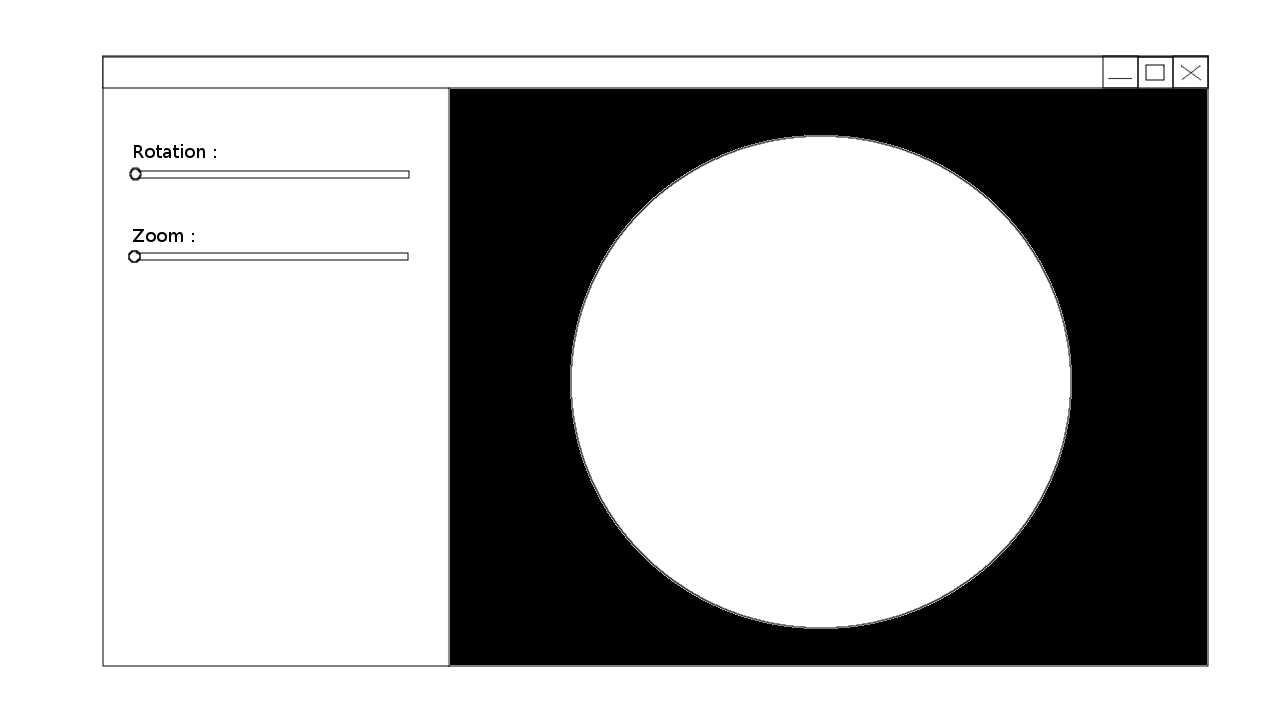
\includegraphics[width=\linewidth]{img/interface_seekbar.png} \end{center}
        \caption{\label{itf_seekbar} Prototype imagée de l'interface utilisateur avec seekbar (dépréciée)}
        \end{figure}
    
    \newpage
        \subsubsection{Effectuer une rotation du point de vue autour de la planète} 
        
        Il faut permettre à l'utilisateur de visualiser la planète sous différents angles.
        Pour cela, il doit être possible de tourner, se déplacer assez précisément autour de la planète.
        
        Un point de vue sera définit par une "caméra" qui se déplacera dans l'espace vectoriel (définit plus haut) lors d'un mouvement de la souris pendant que le clic gauche est enfoncé (une alternative faisant l'usage du clavier est envisageable, notamment utilisant les flèches pour déplacer la caméra pas à pas, de manière discontinue).
        
        Cette caméra aura comme point d'encrage le centre de la planète. Elle effectuera donc une rotation orbitale autour de celle-ci. On affectera (si nécessaire) un coefficient de vitesse aux déplacements de la caméra afin d'assurer que l'observation soit précise et agréable.
        
        Tout cela est rendu possible par l'intermédiaire des bibliothèques open source GLM (pour les mouvements vectoriels) et GLFW (pour la fenêtre et les évènements clavier/souris) (pour plus de détails, voir \cite{TutoCamera}).
        
        \subsubsection{Zoom avec vue première personne} 
        Il doit être possible de zoomer (respectivement dézoomer) sur la planète. 
        
        Cela est faisable en rapprochant (respectivement éloignant) la caméra de la planète lors du défilement de la molette à l'aide des bibliothèques citées précédemment.
        
        Lorsque la caméra est suffisamment proche de la planète, l'angle de vue doit changer pour nous permettre de voir l'horizon. On peut alors faire une rotation (comme une tête) pour observer l'environnement. L'idée serait d'empêcher le zoom lorsque l'on est au plus près de la surface de la planète, et après avoir atteint cette limite, ignorer le point d'encrage de la caméra au centre de la planète pour pouvoir orienter la caméra à notre guise et observer librement l'environnement avec les mouvements de souris pendant que le clic gauche est enfoncé (éventuellement avec les flèches pour orienter la caméra de manière discontinue). Dans cet état, la caméra peut faire une rotation sur elle-même mais ne peut plus se déplacer. 
        
        Lors d'un dézoom, la caméra reprend en compte son point d'encrage pour assurer la visualisation orbitale de la planète décrite précédemment.
        
        Toutes ces manipulations de caméra sont réalisables en utilisant les bibliothèques open source citées précédemment (GLM version stable  0.9.9.7 et GLFW version 3.3 qui est la dernière en date et qui gère mieux les entrées de mouvement de la souris).
        \\\\
        Pour la faisabilité du besoin de visualisation, voir \cite{SongHoAhn} (icosphere.zip) et \cite{TutoCamera}.\\

\subsection{Sauvegarder/Charger la planète :}

    \indent L'utilisateur doit avoir la capacité de sauvegarder les modifications appliquées à une planète puis la recharger pour une utilisation ultérieure. Cette sauvegarde peut être fait en gardant les données sous un format spécifique (txt, json, yaml, xml, obj...). La sauvegarde s'effectuera en pressant simultanément les touches CTRL+S. Le chargement d'un fichier de sauvegarde pourra se faire par paramètres de lancement.
    \par Il faut éventuellement se mettre d'accord sur un format de fichier de sauvegarde commun avec l'autre groupe travaillant sur ce même projet.

\subsection{Priorité des besoins fonctionnels}

    Les besoins fonctionnels sont organisés selon l'ordre de priorité suivant :
    \begin{enumerate}
        \item Priorité haute : 
        \begin{itemize}
            \item Définir un repère
            \item Définir l'échelle (système)
            \item Créer la géométrie (sphère)
            \item Implémenter l'algorithme procédurale (rajouter de l'aléatoire)
            \item Définir une structure de données pour les informations des polygones
            \item Afficher la planète
            \item Effectuer une rotation du point de vue autour de la planète
            \item Zoom/Dézoom
        \end{itemize}
        \item Priorité Moyenne :
        \begin{itemize}
            \item Mettre en place le passage de paramètres à l'algorithme
            \item Changer l'angle de vue à la surface de la planète (première personne)
        \end{itemize}
        \item Priorité basse :
        \begin{itemize}
            \item Sauvegarder/Charger la planète
            \item Ajout d'informations supplémentaires (optionnels, au choix)
        \end{itemize}
    \end{enumerate}

\section{Besoins non fonctionnels}
    \subsection{Besoins comportementaux}
        \subsubsection{Rapidité d'affichage}
        
         Il faut d'abord différencier et définir les différents temps qui s'appliquent à ce projet. 
     
         Le temps de génération désigne le temps nécessaire à la génération procédurale de la planète (géométrie et informations générées procéduralement). Il doit être de l'ordre de quelques secondes seulement (5 secondes environ).
         
         Le temps d'affichage désigne le temps nécessaire à l'affichage de la planète dans la fenêtre. Il doit être de l'ordre de la seconde.
         
         Le temps de rafraîchissement désigne le temps entre deux affichages après un mouvement de la caméra. Il doit être de l'ordre de quelque dixièmes ou centièmes de secondes (30 images par seconde) pour avoir une ergonomie de visualisation correcte.
        
        \subsubsection{Compatibilité} \label{Compatibilité}
        
        Le client doit pouvoir l'utiliser sur sa machine, et il faut donc s'adapter à son matériel, n'ayant pas forcément comme machine une configuration du CREMI, qui est celle que nous utiliserons pour développer le logiciel.
        
        Cela induit une compatibilité avec \textbf{Gentoo Linux} et un test de performance sur une configuration proche de la machine visée. La configuration étant la suivante : Processeur Intel(R) Core(TM) i7-3770 CPU @ 3.40GHz, une carte graphique NVIDIA Corporation GF108GL [Quadro 600] ainsi que 16376040 kB de RAM. Tous les outils envisagés ont des performances variables suivant la machine envisagé, c'est donc un \textbf{point critique} à ce projet.
        
        \subsubsection{Graphisme acceptable}
        
        \indent Il faut un certain nombre de polygones pour rendre une visualisation de la planète assez détaillée pour le client (environ 10000 après discussion avec celui-ci). Ce besoin influe de manière importante sur le temps de génération et d'affichage.
  
    
    \subsection{Besoins organisationnels}
        \subsubsection{Choix des outils}
        Au vu des avantages et inconvénients cités précédemment, le choix le plus avisé parmi les outils de rendu 3D se révèle être OpenGL 3.3. (voir \ref{choixoutil}) 
        \subsubsection{Gestion du temps}
        Les tâches prévisionnelles sont représentées sur la figure \ref{gantt} 
         \begin{figure}[!h]
        
            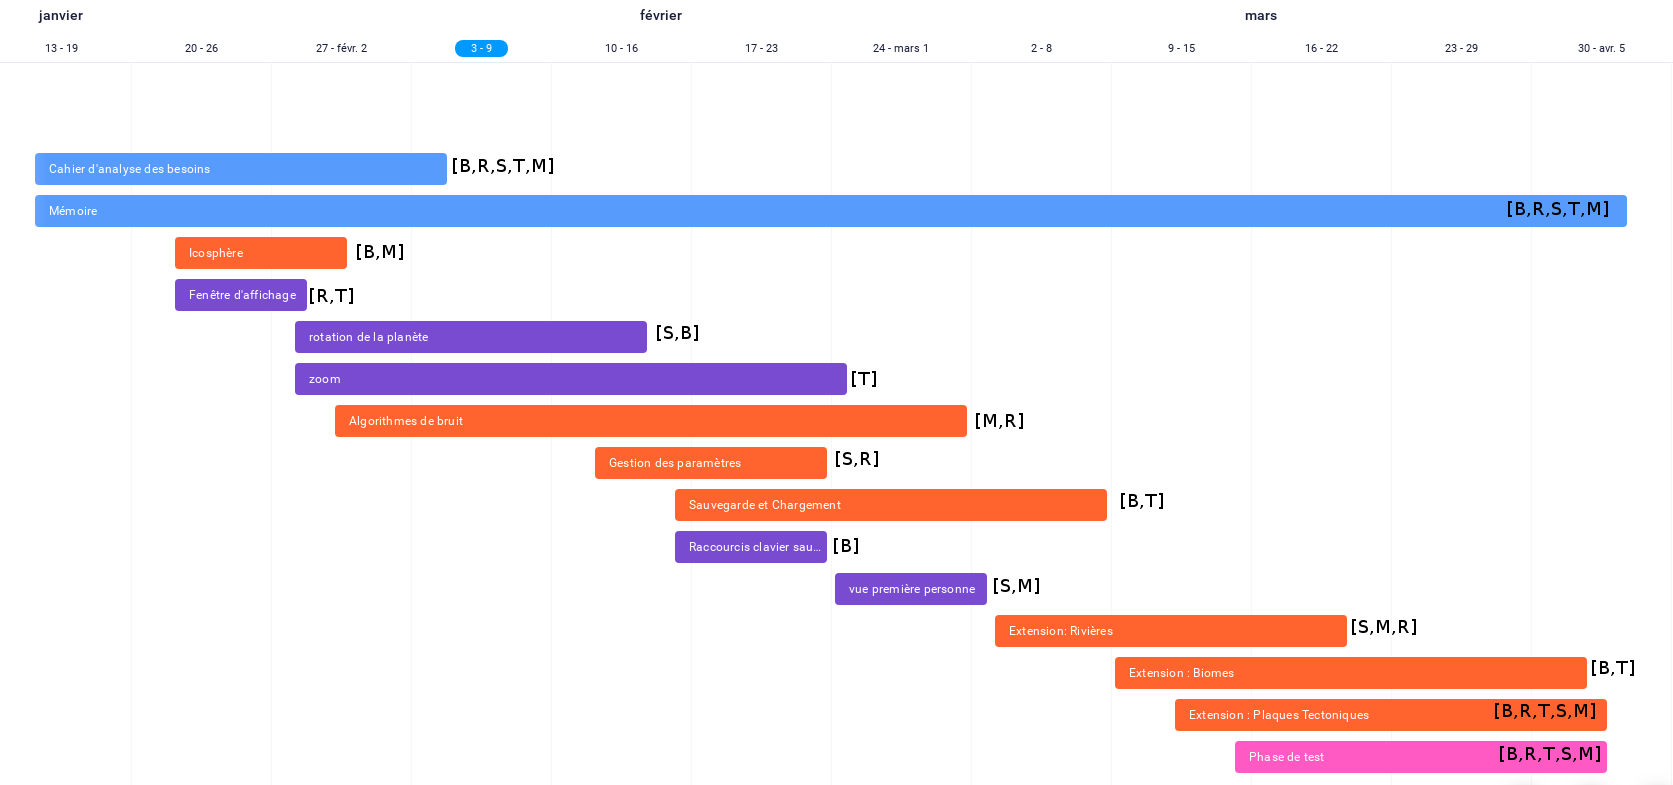
\includegraphics[scale=0.3]{img/gantt.png}
            \caption{\label{gantt}Diagramme de gantt avec les initiales de chaque membre du groupe pour la répartition des taches}
            
        \end{figure}

\section{Risques et parades}

\begin{itemize}
    \item \textbf{Manque de temps} \\
    Le délai de développement est assez réduit et laisse peu de place aux difficultés. Ainsi, il est nécessaire de prioriser certains besoins avant d'autres pour permettre un rendu minimal, c'est-à-dire la génération et visualisation d'une planète avec uniquement des reliefs ainsi que des océans. 
    Le but étant de faire plus que le rendu minimal, il faudra implémenter le plus d'extension possibles (rivières, biomes, plaques tectoniques ...).
    
    \item \textbf{Accès limité à une machine similaire à celle client} \\
    Il sera difficile d'avoir une configuration identique à celle du client pour pouvoir tester les futurs prototypes, cependant il sera possible d'en envoyer régulièrement au client afin d'avoir des retours sur les performances sur la machine cible.
\end{itemize}




\section{Tests}

\subsection{Performance}

Afin de s'assurer du bon fonctionnement du programme sur la machine du client, des tests de performances seront nécessaires. Dans l'idéal, il faudrait tester le programme sur une machine proche de celle du client, notamment au niveau de la carte graphique et du processeur, qui est un facteur déterminant pour le taux de rafraîchissement et le temps de génération respectivement (si nous n'avons pas accès à une machine similaire, soumettre des prototypes au client serait une solution). Il faudrait aussi le faire une dizaine de fois pour s'assurer du bon fonctionnement en moyenne, et sans pics de consommation des ressources.

Un test intéressant aussi pour limiter les paramètres de nos algorithmes serait un test de stress en essayant de créer une planète avec le plus de polygones possible. Cela permettrait de constater les limites mais aussi de récupérer des données sur la marge de performance que l'on peut se permettre.

\subsection{Interface}

Un test de validation pour l'interface sans avoir besoin de donner le programme au client serait de faire un prototype papier, et de le lui soumettre. Cela permettrait aussi de la lui personnaliser à sa guise, et en même temps de vérifier nos scénarios d'utilisation.

Pour vérifier le bon fonctionnement de notre interface, le plus adapté serait d'entrer des interactions aléatoires (principe du "Monkey Test"). Cela permet de s'assurer dans une certaine mesure des comportements de l'utilisateur que l'on n'aurait pas prévu.

\subsection{Génération}

Un test possible pour vérifier que la génération est automatisée est d'utiliser un analyseur d'image afin de vérifier ce que produit notre programme. Plus précisément, rien qu'en créant la forme géométrique de base, une forme ronde d'une couleur unie se départageant du fond devrait être affiché, et facilement identifiable. Cependant l'automatisation de ce test par un analyseur d'image demanderait beaucoup d'efforts et de ressources, et n'est pas adapté aux délais de notre projet. On préférera donc un simple test qualitatif à l'oeil nu.\\

Cependant, il est difficile à partir d'un certain niveau de détail de vérifier à l'oeil nu que la planète soit bien "formée", c'est à dire sans trous, sans faces qui s'intersectent, ou même des normales de faces inversées, ce qui peut résulter en des artefacts ou des anomalies sur la surface de rendu. Un test nécessaire est de vérifier chacun des cas énumérés précédemment.\\

Pour le cas de "trous" dans la sphère, il faut vérifier que toutes les arêtes soit connectées à exactement deux faces. Bien sûr, cela permet juste de déterminer si la forme est pleine. La complexité de ce test étant linéaire au nombre d'arètes, il semble assez intéressant, et permet de détecter le bon raccordement des faces avec peu d'implémentation.\\

Pour le cas où les normales des faces seraient inversées, il suffirait de tester si les dites normales sont vers l'extérieur ou l'intérieur du volume, le centre de la sphère. Avec un simple produit scalaire entre cette normale et le vecteur de la position de la face vers le centre la sphère, ça serait possible et ce en complexité linéaire.\\

Pour le cas de l'intersection des faces, il faudrait vérifier que toutes les faces ne s'intersectent pas entre elles. La complexité étant quadratique, si on intersecte toutes les faces entre elles-mêmes et sachant que le scénario semble peu probable en fin de développement, il serait judicieux de l'utiliser au début du développement et ponctuellement afin de vérifier la forme de base.\\

Pour le test des faces en doubles, une façon de faire moins naïve que d'implémenter le test face à face quadratique, est de vérifier l'arité des sommets de la sphère, c'est à dire, pour une icosphère, vérifier que chaque sommet a bien 5 ou 6 arêtes.
Comme le maillage reste régulier, l'arité des sommets reste dans un certain domaine et cela permet de se ramener à une complexité linéaire de ce problème. \\

Pour vérifier l'aléatoire contrôlé dans nos algorithmes, un test sur plusieurs générations de planètes est recommandé afin de vérifier les probabilités que produisent nos algorithmes. Seulement, ce test permettrait uniquement de vérifier la présence de valeurs aberrantes et n'est pas nécessaire pour le bon fonctionnement du programme.


\newpage

\bibliographystyle{plain}
\section{Bibliographie}
\bibliography{bibliographie}



\end{document}
